% Options for packages loaded elsewhere
% Options for packages loaded elsewhere
\PassOptionsToPackage{unicode}{hyperref}
\PassOptionsToPackage{hyphens}{url}
\PassOptionsToPackage{dvipsnames,svgnames,x11names}{xcolor}
%
\documentclass[
]{article}
\usepackage{xcolor}
\usepackage{amsmath,amssymb}
\setcounter{secnumdepth}{5}
\usepackage{iftex}
\ifPDFTeX
  \usepackage[T1]{fontenc}
  \usepackage[utf8]{inputenc}
  \usepackage{textcomp} % provide euro and other symbols
\else % if luatex or xetex
  \usepackage{unicode-math} % this also loads fontspec
  \defaultfontfeatures{Scale=MatchLowercase}
  \defaultfontfeatures[\rmfamily]{Ligatures=TeX,Scale=1}
\fi
\usepackage{lmodern}
\ifPDFTeX\else
  % xetex/luatex font selection
\fi
% Use upquote if available, for straight quotes in verbatim environments
\IfFileExists{upquote.sty}{\usepackage{upquote}}{}
\IfFileExists{microtype.sty}{% use microtype if available
  \usepackage[]{microtype}
  \UseMicrotypeSet[protrusion]{basicmath} % disable protrusion for tt fonts
}{}
\makeatletter
\@ifundefined{KOMAClassName}{% if non-KOMA class
  \IfFileExists{parskip.sty}{%
    \usepackage{parskip}
  }{% else
    \setlength{\parindent}{0pt}
    \setlength{\parskip}{6pt plus 2pt minus 1pt}}
}{% if KOMA class
  \KOMAoptions{parskip=half}}
\makeatother
% Make \paragraph and \subparagraph free-standing
\makeatletter
\ifx\paragraph\undefined\else
  \let\oldparagraph\paragraph
  \renewcommand{\paragraph}{
    \@ifstar
      \xxxParagraphStar
      \xxxParagraphNoStar
  }
  \newcommand{\xxxParagraphStar}[1]{\oldparagraph*{#1}\mbox{}}
  \newcommand{\xxxParagraphNoStar}[1]{\oldparagraph{#1}\mbox{}}
\fi
\ifx\subparagraph\undefined\else
  \let\oldsubparagraph\subparagraph
  \renewcommand{\subparagraph}{
    \@ifstar
      \xxxSubParagraphStar
      \xxxSubParagraphNoStar
  }
  \newcommand{\xxxSubParagraphStar}[1]{\oldsubparagraph*{#1}\mbox{}}
  \newcommand{\xxxSubParagraphNoStar}[1]{\oldsubparagraph{#1}\mbox{}}
\fi
\makeatother


\usepackage{longtable,booktabs,array}
\usepackage{calc} % for calculating minipage widths
% Correct order of tables after \paragraph or \subparagraph
\usepackage{etoolbox}
\makeatletter
\patchcmd\longtable{\par}{\if@noskipsec\mbox{}\fi\par}{}{}
\makeatother
% Allow footnotes in longtable head/foot
\IfFileExists{footnotehyper.sty}{\usepackage{footnotehyper}}{\usepackage{footnote}}
\makesavenoteenv{longtable}
\usepackage{graphicx}
\makeatletter
\newsavebox\pandoc@box
\newcommand*\pandocbounded[1]{% scales image to fit in text height/width
  \sbox\pandoc@box{#1}%
  \Gscale@div\@tempa{\textheight}{\dimexpr\ht\pandoc@box+\dp\pandoc@box\relax}%
  \Gscale@div\@tempb{\linewidth}{\wd\pandoc@box}%
  \ifdim\@tempb\p@<\@tempa\p@\let\@tempa\@tempb\fi% select the smaller of both
  \ifdim\@tempa\p@<\p@\scalebox{\@tempa}{\usebox\pandoc@box}%
  \else\usebox{\pandoc@box}%
  \fi%
}
% Set default figure placement to htbp
\def\fps@figure{htbp}
\makeatother

\ifLuaTeX
  \usepackage{luacolor}
  \usepackage[soul]{lua-ul}
\else
  \usepackage{soul}
\fi

% definitions for citeproc citations
\NewDocumentCommand\citeproctext{}{}
\NewDocumentCommand\citeproc{mm}{%
  \begingroup\def\citeproctext{#2}\cite{#1}\endgroup}
\makeatletter
 % allow citations to break across lines
 \let\@cite@ofmt\@firstofone
 % avoid brackets around text for \cite:
 \def\@biblabel#1{}
 \def\@cite#1#2{{#1\if@tempswa , #2\fi}}
\makeatother
\newlength{\cslhangindent}
\setlength{\cslhangindent}{1.5em}
\newlength{\csllabelwidth}
\setlength{\csllabelwidth}{3em}
\newenvironment{CSLReferences}[2] % #1 hanging-indent, #2 entry-spacing
 {\begin{list}{}{%
  \setlength{\itemindent}{0pt}
  \setlength{\leftmargin}{0pt}
  \setlength{\parsep}{0pt}
  % turn on hanging indent if param 1 is 1
  \ifodd #1
   \setlength{\leftmargin}{\cslhangindent}
   \setlength{\itemindent}{-1\cslhangindent}
  \fi
  % set entry spacing
  \setlength{\itemsep}{#2\baselineskip}}}
 {\end{list}}
\usepackage{calc}
\newcommand{\CSLBlock}[1]{\hfill\break\parbox[t]{\linewidth}{\strut\ignorespaces#1\strut}}
\newcommand{\CSLLeftMargin}[1]{\parbox[t]{\csllabelwidth}{\strut#1\strut}}
\newcommand{\CSLRightInline}[1]{\parbox[t]{\linewidth - \csllabelwidth}{\strut#1\strut}}
\newcommand{\CSLIndent}[1]{\hspace{\cslhangindent}#1}



\setlength{\emergencystretch}{3em} % prevent overfull lines

\providecommand{\tightlist}{%
  \setlength{\itemsep}{0pt}\setlength{\parskip}{0pt}}



 


\makeatletter
\@ifpackageloaded{caption}{}{\usepackage{caption}}
\AtBeginDocument{%
\ifdefined\contentsname
  \renewcommand*\contentsname{Table of contents}
\else
  \newcommand\contentsname{Table of contents}
\fi
\ifdefined\listfigurename
  \renewcommand*\listfigurename{List of Figures}
\else
  \newcommand\listfigurename{List of Figures}
\fi
\ifdefined\listtablename
  \renewcommand*\listtablename{List of Tables}
\else
  \newcommand\listtablename{List of Tables}
\fi
\ifdefined\figurename
  \renewcommand*\figurename{Figure}
\else
  \newcommand\figurename{Figure}
\fi
\ifdefined\tablename
  \renewcommand*\tablename{Table}
\else
  \newcommand\tablename{Table}
\fi
}
\@ifpackageloaded{float}{}{\usepackage{float}}
\floatstyle{ruled}
\@ifundefined{c@chapter}{\newfloat{codelisting}{h}{lop}}{\newfloat{codelisting}{h}{lop}[chapter]}
\floatname{codelisting}{Listing}
\newcommand*\listoflistings{\listof{codelisting}{List of Listings}}
\makeatother
\makeatletter
\makeatother
\makeatletter
\@ifpackageloaded{caption}{}{\usepackage{caption}}
\@ifpackageloaded{subcaption}{}{\usepackage{subcaption}}
\makeatother
\usepackage{bookmark}
\IfFileExists{xurl.sty}{\usepackage{xurl}}{} % add URL line breaks if available
\urlstyle{same}
\hypersetup{
  pdftitle={Unveiling the Complexity of Food Webs: A Comprehensive Overview of Definitions, Scales, and Mechanisms},
  pdfauthor={Tanya Strydom; Jennifer A. Dunne; Timothée Poisot; Andrew P. Beckerman},
  pdfkeywords={food web, network construction, scientific ignorance},
  colorlinks=true,
  linkcolor={blue},
  filecolor={Maroon},
  citecolor={Blue},
  urlcolor={Blue},
  pdfcreator={LaTeX via pandoc}}



\title{Unveiling the Complexity of Food Webs: A Comprehensive Overview
of Definitions, Scales, and Mechanisms}
\author{Tanya Strydom %
%
\textsuperscript{%
%
1%
}%
; Jennifer A. Dunne %
%
\textsuperscript{%
%
2%
}%
; Timothée Poisot %
%
\textsuperscript{%
3,%
4%
}%
; Andrew P. Beckerman %
%
\textsuperscript{%
%
1%
}%
}
\date{2025-10-07}

\usepackage{setspace}
\usepackage[left]{lineno}
\usepackage[letterpaper]{geometry}

\usepackage[nolists,noheads,markers]{endfloat}
\geometry{margin=2.5cm}

\begin{document}

\thispagestyle{empty}
{\bfseries\sffamily\Large Unveiling the Complexity of Food Webs: A
Comprehensive Overview of Definitions, Scales, and Mechanisms}
\vfil
Tanya Strydom %
%
\textsuperscript{%
%
1%
}%
; Jennifer A. Dunne %
%
\textsuperscript{%
%
2%
}%
; Timothée Poisot %
%
\textsuperscript{%
3,%
4%
}%
; Andrew P. Beckerman %
%
\textsuperscript{%
%
1%
}%

\vfil
{\small
\textbf{Abstract:} Food webs are a useful abstraction and representation
of the feeding links between species in a community and are used to
infer many ecosystem level processes. However, the different theories,
mechanisms, and criteria that underpin how a food web is defined, and
ultimately, constructed means that not all food webs are representing
the same ecological process at the same scale. Here we present a
synthesis of the different assumptions, scales, and mechanisms that are
used to define the different ecological networks , leading to a revision
of definitions for different types of networks. Additionally we
explicitly link the different network representations to the broader
methodological approaches (models) that are used to construct them. In
explicitly outlining the assumptions, scales, and mechanisms of network
inference allows for a formal categorisation of how to use networks to
answer key ecological and conservation questions as wel as defining
clear guidelines to prevent unintentional misuse or misinterpretation.
\vfil
\textbf{Keywords:} %
food web, network construction, %
scientific ignorance%
}
\clearpage
\setcounter{page}{1}
\doublespacing
\linenumbers


At the heart of modern biodiversity science are a set of concepts and
theories about species richness, stability, and function (Loreau \& de
Mazancourt, 2013). These relate to the abundance, distribution,
functions, and services that biodiversity provides. Network
representations of biodiversity are increasingly argued to be an asset
to understanding and predicting the impacts of multiple, simultaneous
stress on these core components of biodiversity (Simmons et al., 2021).
Documenting interactions between and among species is thus one of the
fundamental building blocks of community ecology and provide a powerful
abstraction and platform for mathematical and statistical modelling of
biodiversity to make predictions, and to mitigate and manage threats
(Windsor et al., 2023).

However, there is a growing discourse around limitations to the
interpretation and applied use of networks (Blüthgen, 2010; Dormann,
2023). Against this, it is important to evaluate the value and the
limitations of the various network conceptualisations of biodiversity
(Blüthgen \& Staab, 2024). In this perspective we aim to provide an
overview of different \textbf{food web} representations, particularly
how each representation embeds assumptions about the processes that
determine interactions (Section~\ref{sec-process}) about the levels of
organization at which this occurs (\emph{i.e.} the biological,
ecological, spatial/temporal scale) and and the way in which we
construct the resulting networks (Section~\ref{sec-construct}). The
differences among this tri-partite set of assumptions ultimately
influence the nature and scope of inference that can be made from a
given network (Proulx et al., 2005).

Fundamentally, we are talking about an intersection of the type of data
used to construct a network and the underlying theory as to what drives
the resolution and occurrence of interactions between species in those
data. We still lack a clear explanation of the different assumptions and
scale dependent processes that underpin network construction alongside
extensive discussions about the challenges relating to data collection
and observation (\emph{e.g.,} Blüthgen \& Staab, 2024; Brimacombe et
al., 2023, 2024; Moulatlet et al., 2024; Polis, 1991; Pringle \&
Hutchinson, 2020; Saberski et al., 2024). Such an understanding should
deliver an acceleration in capacity to more effectively predict the
impact of multiple stressors on biodiverse communities.

In their recent work, Gauzens et al. (2025) showcased a 2+2
decomposition of networks around aggregated versus species level
resolution of nodes and around potential and realised links among the
nodes. Their review delivers valuable insight into the methodologies
used to collect and manage data among the node and link differentiation.
It also delivers an overview of the scale and types of questions that
are associated with each category of differentiation.

Here we provide a complementary perspective focused on concepts, models,
and theory, in contrast to the data driven breakdown in Gauzens et al.
(2025) (e.g.~their Tables 1 and 2). Our approach delivers a hierarchical
perspective on network construction based on a gradient from
feasibility, capturing the concept of metawebs and Gauzen et al's
`potential' webs, through to realised webs as in Gauzens' et al.~In
contrast to their 2 + 2 decomposition (their Fig 1), our perspective
showcases nested ecological scales and processes that derive from shifts
in the assumptions and theories embedded along this gradient. This
includes classic ecological `aggregations' such as
functional/phylogenetic groups through to species, populations and
individuals, unique perspective on how space and time intersect with
node and link resolution, refined insight into which networks are
derived by induction vs.~deduction and a revealing of a core transition
between assumptions about how links are derived based on evolutionary
vs.~ecological theories.

In the following sections we provide a scene-setting review of nodes and
edges (links) in networks before aligning various processes that
determine interactions with the different network representations.
Ultimately, we provide a unique perspective on the nested hierarchy of
processes that govern transitions from meta-webs to realised webs. We
finish with a refined and nuanced alignment of models/representations
and key questions in biodiveristy science in the anthropocene.

\section{Setting the Scene: The Not So Basics of Nodes and
Edges}\label{sec-anatomy}

Networks in ecology have multiple uses, representing an `object' from
which inferences can be made. For example, a network is needed to make
inference specifically about the structure of communities. The structure
of networks - their topology - have a long history reflecting core
theory about energy flow {[}Lindeman etc{]}, function {[}REF{]} and even
stability {[}REF{]}. Networks are thus required as the response variable
in evaluating ecological theory and statistical models of `generative
processes' giving rise to such structure {[}REF{]}. Such structure is
now commonly used to compare communities along environmental gradients
{[}REF{]}. Networks and their topology are also used as a platform for
evaluating `downstream' responses to stressors such as evaluating
patterns of secondary extinction {[}REF{]}. Finally, they are commonly
used as a platform for implementing mathematical models of community
dynamics {[}REF{]}; delivering inference about stability, function,
invasive species, climate change, contaminants, and secondary
extinction, to name a few applications {[}REF{]}. Against this backdrop
of multiple research agendas, the definition of `edges' and `nodes', and
the levels of organisation at which they are defined, take many forms
(Moulatlet et al., 2024; Poisot, Stouffer, et al., 2016), each of which
encode a series of assumptions within a network. Here we introduce a
perspective on these baseline assumptions.

\subsection{How do we define a node?}\label{how-do-we-define-a-node}

Although this may seem elementary that a node should represent a
(taxonomic) species, the reality is that nodes often represents
non-taxonomic units such as a trophic species (\emph{e.g.,} Yodzis
(1982); Williams \& Martinez (2000)), a feeding guild (\emph{e.g.,}
García-Callejas et al., 2023), or a segregation of species by life
stages (\emph{e.g.,} Clegg et al., 2018). Such granularity and variation
is often defined as aggregation. Such aggregation can limit the ability
to make species (taxonomic) specific inferences (\emph{e.g.,} does
species \(a\) eat species \(b\)?). It can also affect the estimates of
degree distributions and more specifically generality and vulnerability
in networks (in/out degree). These metrics are central to inference
about the structure and complexity of networks(Beckerman et al., 2006;
Clegg et al., 2018). Finally, aggregation makes it challenging to use
networks in `downstream analyses' of, for example, extinction or
invasions as the identity of species and the consequences of their
losses can be hidden. Despite these issues, there are justifications for
representing nodes as aggregated units. Most prominent relates to when
the distribution of the links between aggregated nodes may be more
meaningful in terms of understanding or generalising about energy flow
and distribution within the system {[}REF{]}.

\subsection{What is captured by an
edge?}\label{what-is-captured-by-an-edge}

In order to break down the definitions of an edge, it is important to
introduce the concept of \emph{potential} versus \emph{realised} links:
potential links reflect feasibility while realised links are connected
to flux of some currency (typically energy; see below for more detail).
Links within food webs are thus a representation of either potential
links between species or fluxes within a system \emph{e.g.,} energy
transfer or material flow as the result of the feeding links between
species {[}Lindeman (1942); Proulx et al. (2005){]}Pringle (2020). Edges
can thus correspond to different `currencies' (Gauzens et al., 2025).
There is also a myriad of ways in which the links themselves can be
specified. Links between species can be treated as present or absent
(\emph{i.e.,} binary), may be defined as probabilities (Banville et al.,
2025; Poisot, Cirtwill, et al., 2016) or by continuous functions which
further quantify the strength of an interaction (Berlow et al., 2004).
How links are specified thus requires intersecting both the currency
being modelled and their specification. For example, feasibility is
unlikely to accommodate flux, but does align with binary or probability
representations. Taking a food web that consists of links representing
feasible interactions among a collection of species will be meaningless
if one is interested in understanding the flow of energy through the
network as the links are not environmentally/energetically constrained.

\subsection{Network representations}\label{sec-representation}

Against these definitions of nodes and edges, networks fall into two
major `types': metawebs, traditionally defined as all the
\emph{potential} interactions for a specific species pool (Dunne, 2006);
and realised networks, which is the subset of interactions in a metaweb
that are \emph{realised} for a specific community at a given time and
place. The fundamental differences between these two network
representations are the spatial and temporal scale at which they are
constructed, and the associated processes that are assumed to drive
pattern at these scales.

A metaweb is, at its core, a list of \emph{feasible} interactions
between pairs of species. The feasibility for a given pair is derived
from the complementarity (phylogenetic relationships) of their traits,
typically aligned with feeding. Feasibility can be further refined by
\emph{co-occurrence} leading to the transition from a \emph{global} to
\emph{regional metaweb}. Metawebs thus provide a means to identify
evolutionarily plausible links, regionally plausible interactions, the
set of ecologically possible, \emph{i.e.,} forbidden, links (Jordano,
2016b), and ultimately a definition of the plausible \emph{complete}
diet of a species (Strydom et al., 2023).

In contrast, realised networks are typically more localised in space and
time, and the links between species are contingent on the co-occurrence
of species, the role of the environment, and mechanisms of diet choice.
Fundamentally this means that the presence/absence of a link is the
result of the `behaviour' of the species and even when the realised
network is presented as a binary matrix, the edges imply a function is
available to define the strength of an interaction. A realised network
is therefore not simply the downscaling of a metaweb to a smaller scale
(\emph{e.g.,} moving from the country to the 1x1 km\textsuperscript{2}
scale based on fine-scale species co-occurrence). Instead, realised webs
capture processes that determine the realisation of an interaction and
flows of energy in a community. Specifically, in realised webs, the
definition of an edge shifts from being determined by feasibility to
that of choices and consequences that centre around energy. If one were
to take the same community of species and constructed both a metaweb and
realised network the two networks might have the same species but would
be structurally different, owing to the differences in the `rules'
constraining the presence of links. This distinction between metawebs
and realised webs leads to a further insight. Links that are absent in a
metaweb can conceptually (although not always practically) be treated as
being truly absent. However, links that are absent in a realised network
cannot be considered as truly absent but rather as absent due to the
broader environmental/community context.

\section{From Nodes and Edges to Process and
Constraints}\label{sec-process}

In the previous section we discussed how the definition of nodes and
edges, representing different scales and processes, lead to the concept
of a metaweb and a realised web. The fundamental take-homes are that
nodes vary in their resolution, edges vary in what kind of process they
represent and the intersection of these, defined by meta- vs.~realised
webs, underpins distinct lines of enquiry and constraints on the type of
inference we can make with networks. Here we reveal five core
constraints across evolutionary and ecological scales that further
delineate the transition from meta- to realised webs, exposing processes
that determine the nature of links among nodes: evolutionary
compatibility, co-occurrence, abundance, diet choice, and non-trophic
interactions Figure~\ref{fig-process}.

\begin{figure}

\centering{

\pandocbounded{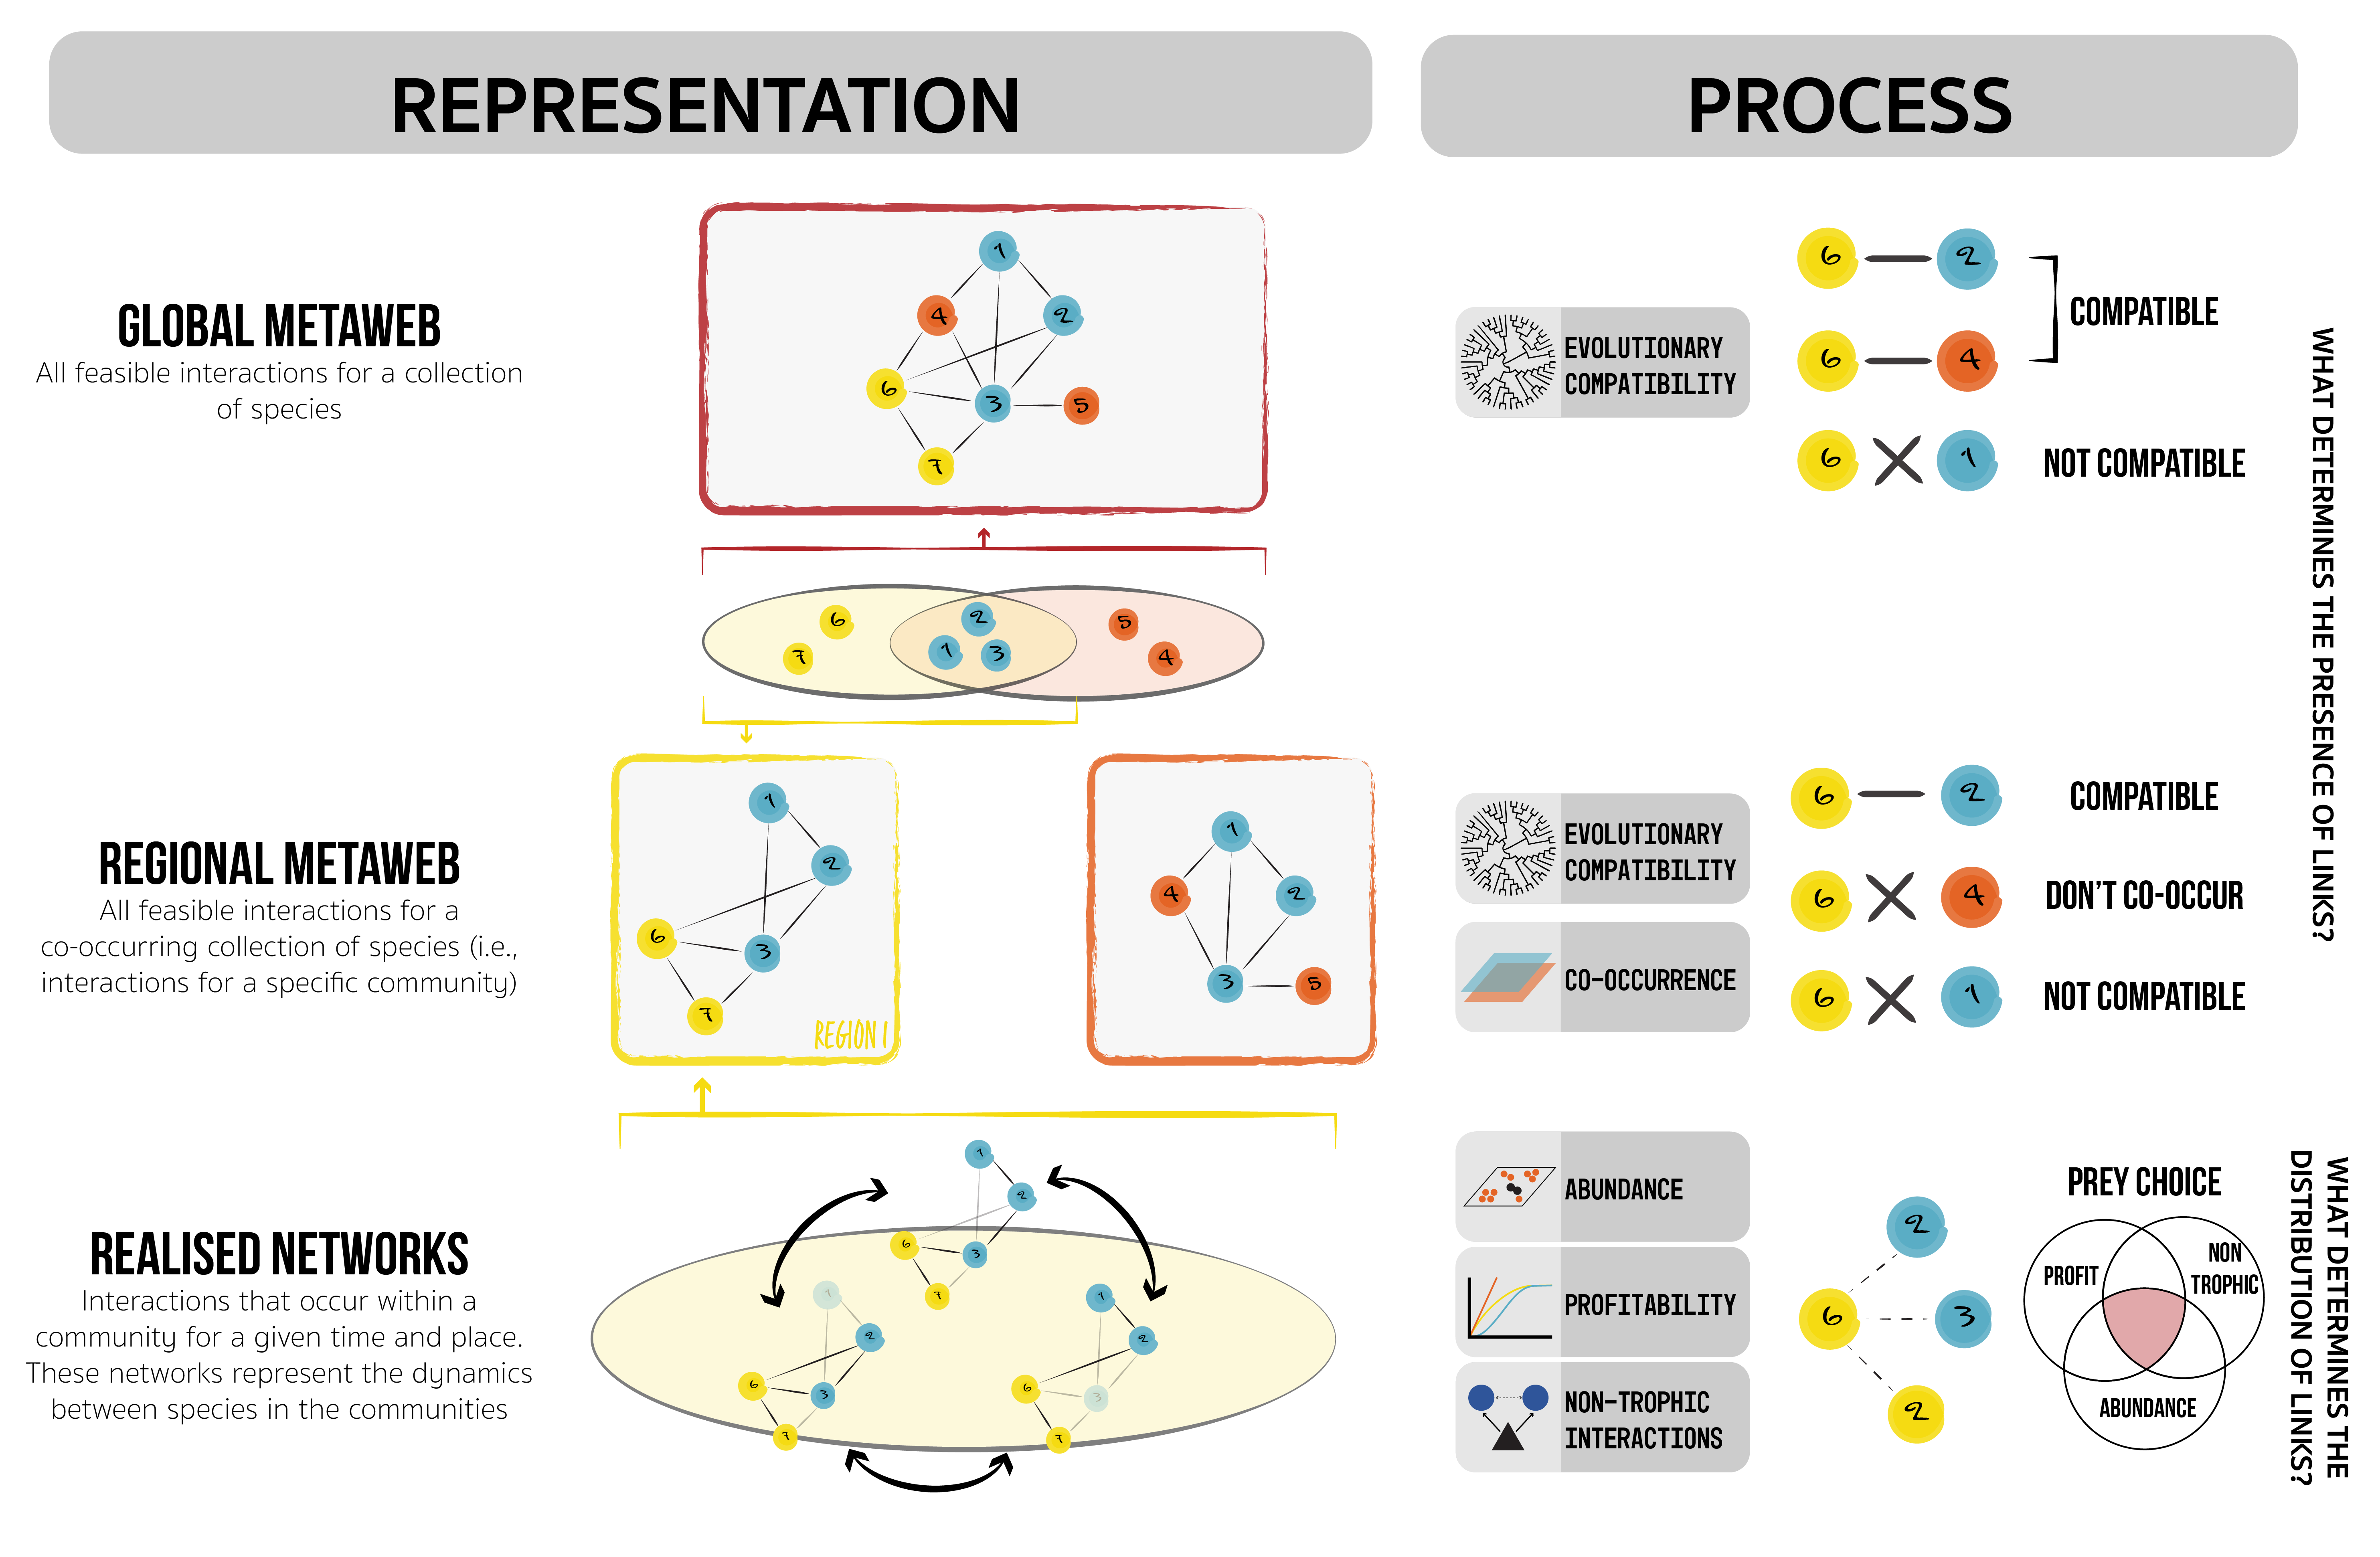
\includegraphics[keepaspectratio]{images/anatomy.png}}

}

\caption{\label{fig-process}Aligning the various processes that
determine interactions (right column) with the different network
representations (left column). First, we start with a \textbf{global
metaweb} this network captures all possible interactions for a
collection of species in the global context. However, within the global
environment different species occur in different regions (region one =
yellow and region 2 = orange), and it is possible to construct two
different metawebs (\textbf{regional metawebs}) for each region by
taking accounting for the co-occurrence of the difference species - as
shown here we have two regions with some species that are found in both
regions (blue) and others endemic to either region one (yellow) or
region two (orange). However even within a region we do not expect all
interactions to be realised but rather that there are multiple
configurations of the regional metaweb over both space and time. The
`state' of the different \textbf{realised networks} is ultimately
influenced not just by the co-occurrence of a species pair but rather
the larger community context such as the abundance of different species,
maximisation of energy gain, or indirect/higher order interactions.}

\end{figure}%

\subsection{Processes that determine the feasibility of an
interaction}\label{sec-process-feasibility}

Evolutionary compatibility and co-occurrence are the two principle
processes that `act' at the species pair of interest and define
feasibility. The scale of inference and set of processes embodied in
these two constraints typically combine to define a `list' of
interactions that are viable/feasible and defined strictly as
present/absent. Reflecting on the previous section, nodes are typically
species and rules defining edges are defined by trait complementarity
(phylogenetic) and/or co-occurrence. Here we provide more insight into
each process.

\textbf{Evolutionary compatibility}

This constraint is defined by shared (co)evolutionary history between
consumers and resources (Dalla Riva \& Stouffer, 2016; Gómez et al.,
2010; Rossberg et al., 2006; Segar et al., 2020) which is manifested as
`trait complementarity' between two species (Benadi et al., 2022). In
this body of theory, the consumer has the `correct' set of traits that
allow it to chase, capture, and consume the resource. Interactions that
are not compatible are defined as forbidden links (Jordano, 2016b);
\emph{i.e.,} they are not physically possible and will \emph{always} be
absent within a network.

Networks do not properly arise from models based on this constraint.
Instead, interacting species pairs are defined and these are represented
as binary (possible vs forbidden) or probabilistic (Banville et al.,
2025). For example, in the metaweb constructed by Strydom et al. (2022)
probabilities are quantified as the confidence of a specific being
\emph{possible} between two species. A network constructed on the basis
of evolutionary compatibility is conceptually aligned with a `global
metaweb', and gives us information as to the global feasibility of links
between species pairs despite the fact that they do not co-occur (see
Figure~\ref{fig-process}).

\textbf{(Co)occurrence}

The co-occurrence of species in both time and space is a fundamental
requirement for an interaction between two species to occur (at least in
terms of feeding links). Although co-occurrence data alone is
insufficient for building an accurate and ecologically meaningful
representation of \emph{feeding links} (Blanchet et al., 2020), it is
still a critical process that determines the realisation of a feeding.
Knowledge on the co-occurrence of species allows us to spatially
constrain a global metaweb to reflect regional metawebs (Dansereau,
Barros, et al., 2024). In the context of Figure~\ref{fig-process} this
would be the metawebs for regions one and two.

We reinforce that these two constraints don't deliver a network
\emph{per se,} but a list of feasible species pairs. Although it is
possible to build a network from the list of interactions generated by
these constraints, it is important to be aware that the structure of
this network is not constrained by any community context: just because
species are able to interact does not mean that they will (Caron et al.,
2024; Poisot et al., 2015).

\subsection{Processes that realise
networks}\label{sec-process-realisation}

In contrast to the above, here we highlight three processes that
influence the \emph{realisation} of an interaction between species and
thus form the conceptual basis for realised networks. As we show in
Figure~\ref{fig-process}, a `truly realised' network is the product of
properties of the community (\textbf{abundance} and \textbf{non-trophic
interactions}) and the individual (\textbf{diet choice}). This
represents a conceptual shift from considering the feasibility for
species pairwise interactions to considering the edge as a
representation of energy flow. Such a transition requires information
about how the community, the environment and the individual
\emph{constrains} network topology as defined by consumer choice
(Quintero et al. (2024), Section~\ref{sec-representation})

\textbf{Abundance}

Abundance as a realising process emerges from a null model for energy
acquisition: organisms feeding randomly will consume resources in
proportion to their abundance (Stephens \& Krebs, 1986). Here, abundance
of different prey species influences the distribution of links in a
network (Vázquez et al., 2009) by defining a preference linked to
individuals among species meeting (Banville et al., 2025; Poisot et al.,
2015). Abundance data, linked to a derived metaweb delivers a foundation
ruleset that can define the distribution and strength of links. Of note,
however, is that such abundance constrained interactions are not
necessarily contingent on there being any compatibility between species
(E. Canard et al., 2012; Momal et al., 2020; Pomeranz et al., 2019).

\textbf{Diet choice}

It is well established that consumers make more active decisions than
eating items in proportion to their abundance (Stephens \& Krebs, 1986).
Ultimately, consumer choice is underpinned by an energetic cost-benefit
framework centred around profitability and defined by traits associated
with finding, catching, killing, and consuming a resource (Smith et al.,
2021; Wootton et al., 2023). Energetic constraints are invoked to
construct networks in a myriad of ways (\emph{e.g.,} Beckerman et al.,
2006; Cherif et al., 2024; Pawar et al., 2012; Portalier et al., 2019).

In contrast to metaweb `construction' from a list of pairwise
interactions, these methods deliver a realised web directly and as an
emergent property of node behaviour. We also here make a distinction,
developed below, with models like the Niche Model, where diet choice is
implicit in it's probabilistic network generating function, but it is
working to replicate the \emph{expected} structure of the network and
this structure does not emerge from node-based rules. Note that we
select diet choice as a term to capture rules linked to optimal foraging
(Pyke, 1984) and metabolic theory (Brown et al., 2004); it is a sensible
`umbrella concept' for capturing the energetic constraint on of the
distribution and strength of interactions.

\textbf{Non-trophic interactions}

We include non-trophic interactions (see Miele et al., 2019) here not as
a determinant of links, but a modifier of them - they are the community
context above and beyond co-occurrence and abundance. Non-trophic
interactions include competition for space, predator interference,
refuge provisioning, recruitment facilitation as well as non-trophic
effects that increase or decrease mortality. These interactions (Ings et
al., 2009) specifically modify either the realisation or strength of
trophic interactions (Golubski \& Abrams, 2011; Kamaru et al., 2024;
Pilosof et al., 2017; Staniczenko et al., 2010) and represent direct
(e.g., predator \(a\) outcompetes predator \(b\)) and indirect (e.g.,
mutualistic/facilitative interactions) mechanisms. They operate on the
realisation of a network by altering the fine-scale distribution and
abundance of species and relative contributions of direct and indirect
effects to biomass, persistence, stability and the functioning of the
communities (Buche et al., 2024; Kéfi et al., 2012, 2015; Miele et al.,
2019).

\textbf{are these strictly modifiers of realised networks? - because we
class them as community context with co-occurrence, a modifier of
feasible networks\ldots.}

\section{Network construction}\label{sec-construct}

The above five processes are central to understanding the assumptions
inherent in building different types of networks. Each of the processes,
or combinations thereof, deliver a unique set of boundary conditions on
what a network represents and can be used for. Here we build on the
introduction of these five processes to further categorise the
approaches to constructing networks. In doing so also introduce more
detail on a variety of methodologies used to construct networks.

\subsection{Why construct networks?}\label{why-construct-networks}

Networks are a representation of biodiversity. In a perfect world, we
might know about all interactions. However, the empirical collection of
interaction data is both costly and challenging to execute (Jordano,
2016a, 2016b; Poisot et al., 2021). In the absence of robust empirical
data, we construct models that facilitate interpolation and gap-filling
of existing empirical datasets (\emph{e.g.,} Biton et al., 2024; Dallas
et al., 2017; Poisot et al., 2023; Stock et al., 2017), predict the
feasibility of interaction among pairs of species, or directly predict
network structure (see Strydom, Catchen, et al., 2021 for a broader
discussion).

They are unique in delivering more than just estimates of species
richness. As note in the introduction, a network embodies the organising
structure of biodiversity and allows numerous opportunities for
`downstream' analysis, including the comparison of structures,
estimation of energy flux or extinction dynamics and ultimately form the
structural inputs to dynamical systems models that facilitate ecological
and conservation relevant inference about
productivity-diversity-stability-function relationships (Danet et al.,
2024) in space and time. But making such inferences requires careful
attention to one or more of the processes discussed in
Section~\ref{sec-process}.

\subsection{Construction through induction}\label{sec-construct-induct}

Constructing feasible or realised networks can be framed as an
`inductive reasoning' process where insight and generalisation arises
from a set of observations and relationships. Inductive reasoning as a
foundation for network construction is implemented through node- and
network levels. When applied at the node level, species specific
networks are created and judge by their association with expected
feeding interactions. When applied at the network level, networks are
judged by their structural properties per se.

\subsubsection{Species specific networks: construction through node
level
induction}\label{species-specific-networks-construction-through-node-level-induction}

Constructing feasible networks and facilitating the interpolation or
gap-filling of existing empirical datasets on sets of species
interactions can be framed as an `inductive reasoning' process where
insight and generalisation arises from a set of observations and
relationships about feeding. All methods in this inference space rest on
a set of three assumptions: there are a set of `feeding rules' that
underpin interaction feasibility (Morales-Castilla et al., 2015); these
rules are phylogenetically conserved (Bramon Mora et al., 2018; Dalla
Riva \& Stouffer, 2016); they can be specified by matching the traits
between consumer and resource.

Evolutionary compatibility and co-occurrence constraints, the foundation
theory for feasible networks, and have delivered insight in many ways.
They have been critical to the construction of `first draft' networks
for communities for which we have no interaction data (Strydom et al.,
2022). They are also central to interpolation in data poor regions and
predicting interactions for `unobservable' communities \emph{e.g.,}
prehistoric networks (Dunhill et al., 2024; Fricke et al., 2022; Yeakel
et al., 2014) or future, novel community assemblages (Van der Putten et
al., 2010). Furthermore, they have the capacity to evaluate a role of
interactions among species relative to their distribution by accounting
for the role of the environment and the role of species interactions
(Gravel et al., 2019; Higino et al., 2023; Pollock et al., 2014).There
are substantial data requirements for these approaches including expert
knowledge, species traits and phylogenetic relationships and/or
interaction data on related species or communities.

Feeding rules are defined in multiple ways. The determination of the
feeding rules can be defined \emph{a priori} based expert knowledge
opinions. Typically this is done on a `trait matching' basis. An example
are the paleo food web models of Shaw et al. (2024) and Roopnarine
(2017) that specify a series of rules for a set of traits and
interactions are deemed feasible if all conditions are met.
Alternatively the body size ratio between the consumer and resource is
often used (\emph{e.g.,} Gravel et al., 2013; Rohr et al., 2010), with
the idea that consumers will only utilise a resource with a body size is
less than or equal to their own. However, work from Van De Walle et al.
(2023) seems to suggest that adding morphological traits in addition to
body size ratio improves model performance.

Rules are also defined by correlating real world interaction data with
suitable ecological proxies for which data is more widely available
(\emph{e.g.,} traits) using some sort of binary classifier (see Pichler
et al. (2020) for an overview). These include generalised linear models
(\emph{e.g.,} Caron et al., 2022), random forest (\emph{e.g.,} Llewelyn
et al., 2023), trait-based k-NN (\emph{e.g.,} Desjardins-Proulx et al.,
2017), and Bayesian models (Cirtwill et al., 2019; \emph{e.g.,} Eklöf et
al., 2013).

Finally, graph embedding uses the structural features of a known network
to infer the position of species in an unknown network through the
decomposition of the interaction onto the embedding space. This
decomposition relies on a combination of ecological proxies
\textbf{(e.g.~???)} in conjunction with known interactions to infer the
latent values of species \textbf{What is a latent value of a species
with respect to inferring interactions?}. See Strydom et al. (2023) for
a detailed review of methods and Strydom et al. (2022) for a specific
example.

\subsubsection{Species agnostic networks: construction through structure
induction}\label{species-agnostic-networks-construction-through-structure-induction}

Networks in this category are generated rules that create non-random
(\textbf{note that this is irritated by the Random models paragraph
below; do we need that? The stochastic models are the `real' version of
this type of network?}) networks that reflect empirical knowledge of
ecological network structures and evaluated by matching predictions to
this \emph{expected} structure of the network(s). The determination of
links between species is only implicitly linked to properties of the
nodes (\textbf{see ADBM 5 rules}). This means these networks are usually
not species specific. Although these models are data input light, often
requiring only species richness and an estimate of the number of
expected links, they make clear assumptions regarding what the
expectations are for network structure. These are some of the most
commonly used network generation tools (e.g.~the Niche model REF). There
are two sub-categories of these species agnostic networks:

Random network models (Bascompte et al., 2003; \emph{e.g.,} Erdős \&
Rényi, 1959; Fortuna \& Bascompte, 2006) represent a `process free'
model. These models are not explicitly tied to a process discussed in
Section~\ref{sec-process}, rather links are randomly distributed among
nodes. Although these models lack real world tractability (Bascompte,
2007) they are often used as a `null hypothesis' to ask questions about
network structure (\emph{e.g.,} Banville et al., 2023; Strydom, Dalla
Riva, et al., 2021).

Stochastic network models use a probabilistic rule-set about diet choice
and niche breadth to reflect fundamental ideas of foraging biology.
\textbf{RATHER THAN ALLESINA, I'D SUGGEST PRESENTING THE 5 RULES IN THE
ADBM EXPLANATION OF THE NICHE MODEL} These models that are based on the
compartmentation and acquisition of energy for species at different
trophic levels (Allesina \& Pascual, 2009; Krause et al., 2003) and that
network structure can be determined by distributing interactions along
single dimension {[}the `niche axis'; Allesina et al. (2008){]}.
Typically these models parametrise some aspect of the network structure
(although see Allesina \& Pascual, 2009 for a parameter-free model).
These models include the most commonly used network generator, the Niche
model (Williams \& Martinez, 2000), as well as the original Cascade
model (Cohen et al., 1990) and the derived Nested hierarchy model
(Cattin et al., 2004). These models often form the basis for dynamic
models \emph{e.g.,} the allometric trophic network (Brose et al., 2006;
Schneider et al., 2016) and bioenergetic food web models (Delmas et al.,
2017).

\subsection{Construction through
deduction}\label{construction-through-deduction}

In contrast to the above approaches centred on feasibility, relised
networks via methods reflecting abundance and diet choice typically rely
on deductive reasoning and have a unique agenda to those above. In
contrast to the inductive methods, inference about a realise network
follows from a set of premises defining generative processes, often
referred to as mechanisms. Typically, models that embed abundance and
diet choice constraints reference theory that allows inference about the
distribution and strength of interactions. Such models are `network
topology generators' and have a strong representation in research
comparing network structures along environmental gradients and
delivering inference about extinctions and energy flux. They also
provide the structural backbone for dynamical systems modelling to
address questions about stability-structure-productivity-function
relationships, secondary extinction dynamics, species invasion and
climate change. There are two broad group of models in this deductive
category.

\subsubsection{Species-specific
networks}\label{species-specific-networks}

These models capture the behaviour of the nodes by explicitly taking
into account the properties of the different species in the community.
Which means that there is a degree of variance in which links are
predicted between species unlike the more `static' predictions made by
inductive models. However, these networks are `costly' to construct in
real world settings (requiring data about the entire community, as it is
the behaviour of the system that determines the behaviour of the part)
and also lack the larger diet niche context afforded by metawebs.

Neutral networks are built on the assumption that foraging decisions are
tied \emph{only} to the abundance of species within the community (E. F.
Canard et al., 2014; Krishna et al., 2008). Here links are soley
determined by the relative abundance of the different species in the
community. Although it is highly unlikely that abundance is the only
determaninant of interactions work by Pomeranz et al. (2019) showcases
how these neutral processes can be used in conjunction with inductive
models to construct more refined/localised networks.

There is a broader group of models that focus on determining
interactions in terms of energetic constraints on diet breadth, often
using the ratio of consumer-resource bodysize as a proxy for capturing
the energetic constraints of feeding. Models such as those developed by
Portalier et al. (2019) and Wootton et al. (2023) are similar to the
mechanistic approaches discussed in Section~\ref{sec-construct-induct},
however instead of determining interactions based on mechanistic
feasibility it is rather constrained by the energetic cost of predation.
Note that although these models do not place any explicit constraints on
the expected structure of the network, the links should still be
considered as `realised' owing to the energetic constraint placed on
links. A different subset of diet models (\emph{e.g.,} Beckerman et al.,
2006; Petchey et al., 2008) use a diet choice approach, however similar
to the stochastic network models they also embed assumptions on network
structure. Thus these models predict both interactions and network
structure simultaneously, although they would benefit in being refined
by more explicitly accounting for trait-based (\emph{i.e.,} feasibility)
paramterisation (Curtsdotter et al., 2019).

\section{Making Progress with Networks}\label{sec-progress}

\textbf{THIS SECTION NEEDS WORK. THE FIRST TWO SENTENCES SAY TOO MUCH AT
ONCE AND NOT ENOUGH} Our introduction put forward that biodiversity
science is underpinned by a set of concepts and theories about species
richness, stability, and function that help define the abundance,
distribution, functions and services that biodiversity provides (Loreau
\& de Mazancourt, 2013). We have above delieverd a hierarchical
framework encompassing the wide range of ways that biodiversity is
representated as a network. These representations carry assumptions that
foster specific sets of questions (see also Gauzens et al., 2025).

Here we present a range of opportunities that emerge from these
frameworks and the clarity afforded by our classification. Leverging Box
1 details that underscore how specific network representations capture
specific processes, we present two groups of opportunites. First, we
highlight a set that advances specifically our understanding of
ecological theory and provide predictions and generalisations of
emergent properties of ecological communities and ecosystems. Second, we
highlight a set that address aspects of key global challenges facing
humanity where biodiversity is at the core. The latter aims to showcase
how we might transition from simply documenting declines and negative
impacts to using network representations of biodiversity to provide
solutions.

\st{It is probably both this nuance as well as a lack of clear
boundaries and guidelines as to the links between network form and
function (although see Delmas et al., 2019) that has stifled the
`productive use' of networks beyond the inventorying the interactions
between species. Although progress with using networks as a means to
address questions within larger bodies of ecological theory \emph{e.g.,}
invasion biology (Hui \& Richardson, 2019) and co-existence theory
(García-Callejas et al., 2023) has been made we still lack explicit
guidelines as to what the appropriate network representation for the
task at hand would be, and as highlighted in}

\subsection{Making use of the different network
representations}\label{making-use-of-the-different-network-representations}

\textbf{Advancing Ecological Theory}

\begin{itemize}
\tightlist
\item
  ENSEMBLING:: -- Tools that allow us to estimate both the feasibility
  as well as realisation of links: Currently most approaches to
  modelling realised networks fail to explicitly account for any form of
  evolutionary constraint Wootton et al. (2023) and we need to develop
  either an ensemble modelling approach (Becker et al., 2022; Terry \&
  Lewis, 2020) or tools that will allow for the downsampling of metawebs
  into realised networks (\emph{e.g.,} Roopnarine, 2006). -- Is there
  something in generalisable models that `combine' different
  processes/aspects (\emph{e.g.,} using body size as a catch all) versus
  limited models that allow you to unpack things bit-by-bit
  (\emph{i.e.,} process by process). So Wootton et al. (2023) \emph{may}
  (TBD) span the gamut but it lacks the ability to unpack\ldots{}
  Although maybe the terms do?
\item
  MODEL PIECES :: Modelling interaction strength: Although realised
  networks are more closely aligned with \emph{explicitly} capturing
  interaction strength we lack models that allow us to quantify this
  (Strydom, Catchen, et al., 2021; Wells \& O'Hara, 2013).\emph{Is this
  about defining IS in models or model validation or predicting IS as
  emergent property or all of this}
\item
  MODEL-DATA :: How do we validate our predictions?: Progress has been
  made to assess how well a model recovers pairwise interactions
  (Poisot, 2023; Strydom, Catchen, et al., 2021), but we still lack
  clear set of guidelines for benchmarking the ability of models to
  recover structure (Allesina et al., 2008)
\item
  EMERGENT PREDICTIONS - ECOLOGICAL THEORY: Do the decades of insights
  arrived at for stability-diversity-productivity relationships with
  tri-trophic or diamond shaped models hold for complex communities
  (10's-100s) (Danet et al., 2024); How will spatial and temporal
  variation in climate and productivity drive change in complex
  ecosystems. Necessary to move to predicting changes in biodiversity
  per se, ecosystem functions and identifying sensitive and robust
  species and portions of communities.
\item
  REWIRING:: Does rewiring happen and does it deliver robustness?
  Specific sub points to consider here is persistence, especially
  persistence to perturbation. Again, dynamic networks and
  network/community assembly and finally extinctions (Dunhill et al.,
  2024).
\end{itemize}

\textbf{Conservation Applications} - How will novel communities
interact? How will range shifts and invasions result in new/novel
community assemblages. And then also the intentional changes of species
compositions through rewilding. - MULTI-LAYER NETWORKS: -- Can
socioeconomic networks combined with biological networks drive
understanding of externalities? -- Brose et al information networks -
MULTIPLE STRESSOR SENSITIVITY ANALYSIS \emph{using models to identify
most at risk species processes} \emph{using models to identify
driver/stressor to invest in to limit impacts} \emph{using models to
quantify resistance (rivets) and resilience/recovery potential (multiple
states too) }early warning* -- INVASION-EXTINCTION:: When do invasive
species enhance or decimate communities? When do reintroductions work?
(Wooster et al., 2024) -- TEMPERATURE - Are there temperature threshold
to community collapse -- Multiple stressor allocation across networks
(among species; among trophic levels; bioaccumulation) -- Land Use and
Harvesting and Temperature and Contaminants - Can paleoecological data
from deep time hyperthermal events provide sufficient insight into the
targets, pace and recovery times from rapid climate events?

Something about making what we do with networks more tractable in the
applied space? \emph{e.g.,} Dansereau, Braga, et al. (2024)

\begin{figure}

\centering{

\pandocbounded{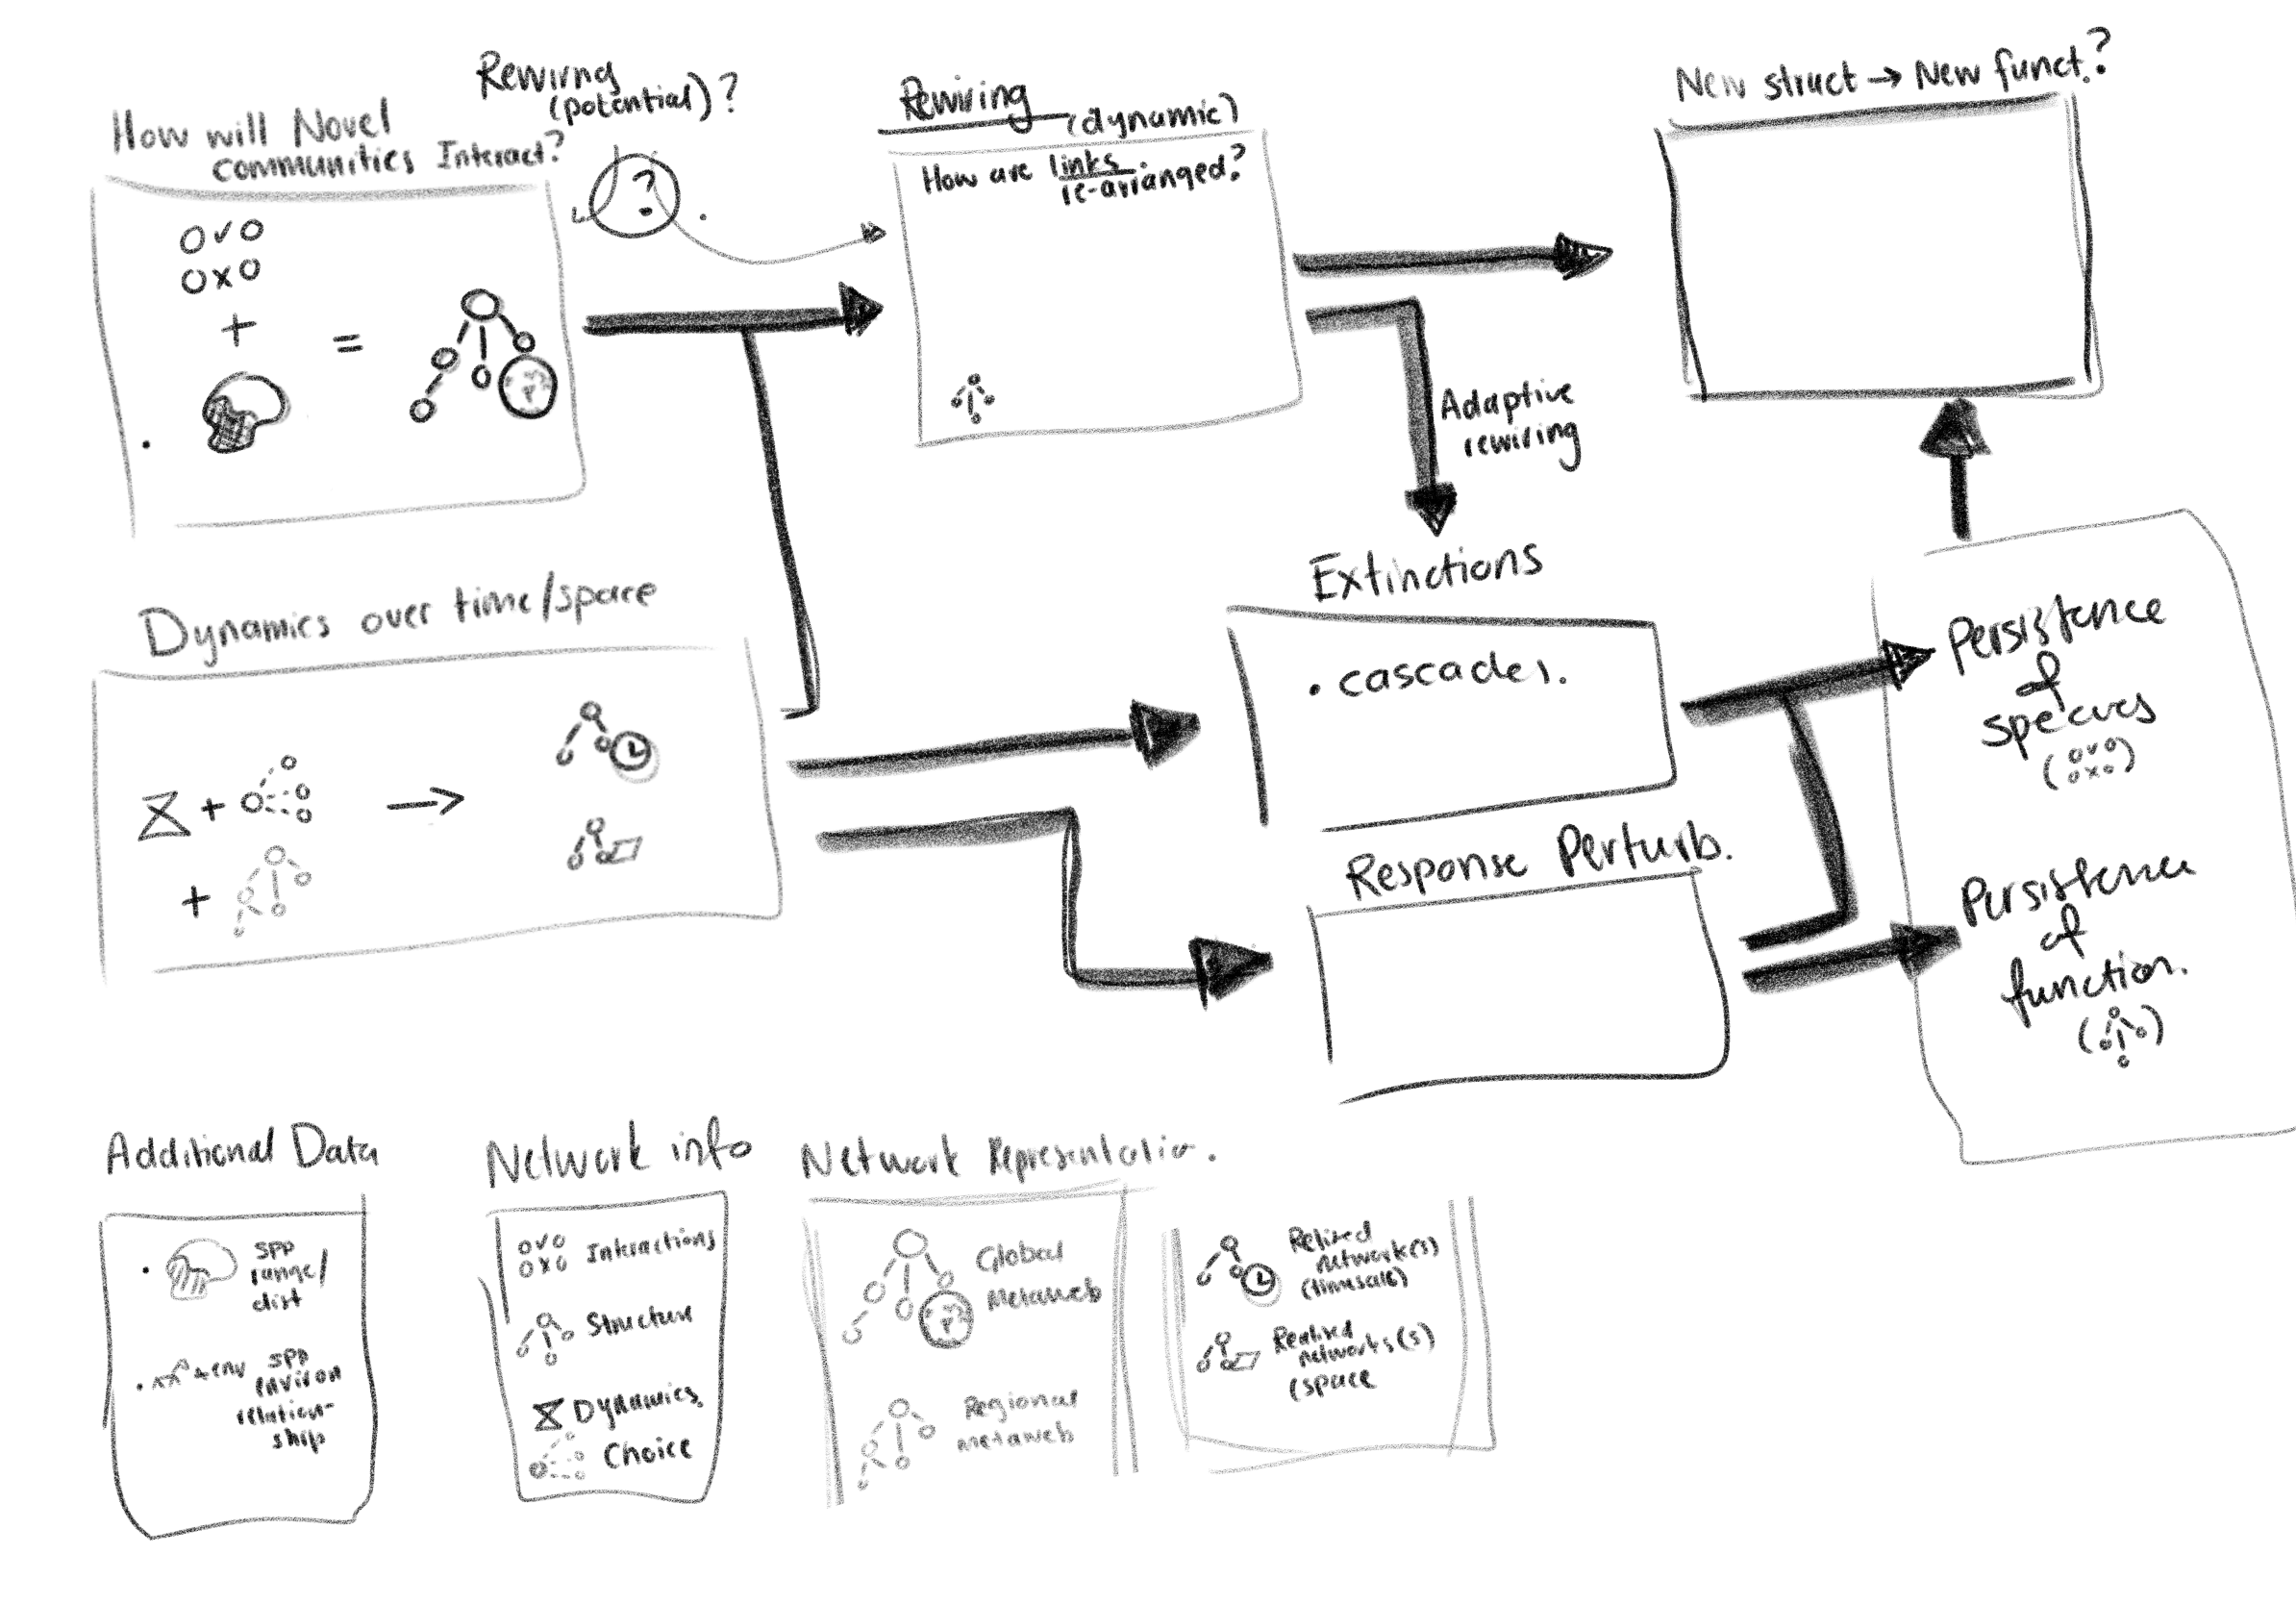
\includegraphics[keepaspectratio]{images/NetworkFuture.png}}

}

\caption{\label{fig-future}Here we highlight some of the outstanding
questions in both network as well as general ecology, as well as some of
the outstanding methodological challenges with regards to constructing
food webs (shown in orange) that we are faced with.}

\end{figure}%

\section{Concluding remarks}\label{concluding-remarks}

Having a clear understanding of the interplay between network
representations and the processes that they are capable of encoding is
critical if we are to understand exactly which networks can be used to
answer which questions. As we highlight in Box 1 the different network
representations have different potential uses and it should be clear
that there is no `best' network representation but rather a network
representation that is best suited to its intended purpose. In providing
a formalisation regards to the assumptions and mechanisms that need to
be explicitly taken into consideration when deciding to use (and
construct) networks we hope to prevent the unintentional misuse or
misinterpretation of networks as well as provide a starting point from
which we can develop a better framework for the applied use of networks
to answer questions that are not only pressing within the field but also
within broader biodiversity science.

\section*{References}\label{references}
\addcontentsline{toc}{section}{References}

\phantomsection\label{refs}
\begin{CSLReferences}{1}{0}
\bibitem[\citeproctext]{ref-allesinaGeneralModelFood2008}
Allesina, S., Alonso, D., \& Pascual, M. (2008). A {General Model} for
{Food Web Structure}. \emph{Science}, \emph{320}(5876), 658--661.
\url{https://doi.org/10.1126/science.1156269}

\bibitem[\citeproctext]{ref-allesinaFoodWebModels2009}
Allesina, S., \& Pascual, M. (2009). Food web models: A plea for groups.
\emph{Ecology Letters}, \emph{12}(7), 652--662.
\url{https://doi.org/10.1111/j.1461-0248.2009.01321.x}

\bibitem[\citeproctext]{ref-banvilleWhatConstrainsFood2023}
Banville, F., Gravel, D., \& Poisot, T. (2023). What constrains food
webs? {A} maximum entropy framework for predicting their structure with
minimal biases. \emph{PLOS Computational Biology}, \emph{19}(9),
e1011458. \url{https://doi.org/10.1371/journal.pcbi.1011458}

\bibitem[\citeproctext]{ref-banvilleDecipheringProbabilisticSpecies2025}
Banville, F., Strydom, T., Blyth, P. S. A., Brimacombe, C., Catchen, M.
D., Dansereau, G., Higino, G., Malpas, T., Mayall, H., Norman, K.,
Gravel, D., \& Poisot, T. (2025). Deciphering {Probabilistic Species
Interaction Networks}. \emph{Ecology Letters}, \emph{28}(6), e70161.
\url{https://doi.org/10.1111/ele.70161}

\bibitem[\citeproctext]{ref-bascompteNetworksEcology2007}
Bascompte, J. (2007). Networks in ecology. \emph{Basic and Applied
Ecology}, \emph{8}(6), 485--490.
\url{https://doi.org/10.1016/j.baae.2007.06.003}

\bibitem[\citeproctext]{ref-bascompteNestedAssemblyPlantanimal2003}
Bascompte, J., Jordano, P., Melian, C. J., \& Olesen, J. M. (2003). The
nested assembly of plant-animal mutualistic networks. \emph{Proceedings
of the National Academy of Sciences}, \emph{100}(16), 9383--9387.
\url{https://doi.org/10.1073/pnas.1633576100}

\bibitem[\citeproctext]{ref-beckerOptimisingPredictiveModels2022}
Becker, D. J., Albery, G. F., Sjodin, A. R., Poisot, T., Bergner, L. M.,
Chen, B., Cohen, L. E., Dallas, T. A., Eskew, E. A., Fagre, A. C.,
Farrell, M. J., Guth, S., Han, B. A., Simmons, N. B., Stock, M.,
Teeling, E. C., \& Carlson, C. J. (2022). Optimising predictive models
to prioritise viral discovery in zoonotic reservoirs. \emph{The Lancet
Microbe}, \emph{3}(8), e625--e637.
\url{https://doi.org/10.1016/S2666-5247(21)00245-7}

\bibitem[\citeproctext]{ref-beckermanForagingBiologyPredicts2006}
Beckerman, A. P., Petchey, O. L., \& Warren, P. H. (2006). Foraging
biology predicts food web complexity. \emph{Proceedings of the National
Academy of Sciences}, \emph{103}(37), 13745--13749.
\url{https://doi.org/10.1073/pnas.0603039103}

\bibitem[\citeproctext]{ref-benadiQuantitativePredictionInteractions2022}
Benadi, G., Dormann, C. F., Fründ, J., Stephan, R., \& Vázquez, D. P.
(2022). Quantitative {Prediction} of {Interactions} in {Bipartite
Networks Based} on {Traits}, {Abundances}, and {Phylogeny}. \emph{The
American Naturalist}, \emph{199}(6), 841--854.
\url{https://doi.org/10.1086/714420}

\bibitem[\citeproctext]{ref-berlowInteractionStrengthsFood2004}
Berlow, E. L., Neutel, A.-M., Cohen, J. E., de Ruiter, P. C., Ebenman,
B., Emmerson, M., Fox, J. W., Jansen, V. A. A., Iwan Jones, J.,
Kokkoris, G. D., Logofet, D. O., McKane, A. J., Montoya, J. M., \&
Petchey, O. (2004). Interaction strengths in food webs: Issues and
opportunities. \emph{Journal of Animal Ecology}, \emph{73}(3), 585--598.
\url{https://doi.org/10.1111/j.0021-8790.2004.00833.x}

\bibitem[\citeproctext]{ref-bitonInductiveLinkPrediction2024}
Biton, B., Puzis, R., \& Pilosof, S. (2024). \emph{Inductive link
prediction boosts data availability and enables cross-community link
prediction in ecological networks}. EcoEvoRxiv.

\bibitem[\citeproctext]{ref-blanchetCooccurrenceNotEvidence2020}
Blanchet, F. G., Cazelles, K., \& Gravel, D. (2020). Co-occurrence is
not evidence of ecological interactions. \emph{Ecology Letters},
\emph{23}(7), 1050--1063. \url{https://doi.org/10.1111/ele.13525}

\bibitem[\citeproctext]{ref-bluthgenWhyNetworkAnalysis2010}
Blüthgen, N. (2010). Why network analysis is often disconnected from
community ecology: {A} critique and an ecologist's guide. \emph{Basic
and Applied Ecology}, \emph{11}(3), 185--195.
\url{https://doi.org/10.1016/j.baae.2010.01.001}

\bibitem[\citeproctext]{ref-bluthgenCriticalEvaluationNetwork2024}
Blüthgen, N., \& Staab, M. (2024). A {Critical Evaluation} of {Network
Approaches} for {Studying Species Interactions}. \emph{Annual Review of
Ecology, Evolution, and Systematics}, \emph{55}(1), 65--88.
\url{https://doi.org/10.1146/annurev-ecolsys-102722-021904}

\bibitem[\citeproctext]{ref-bramonmoraIdentifyingCommonBackbone2018}
Bramon Mora, B., Gravel, D., Gilarranz, L. J., Poisot, T., \& Stouffer,
D. B. (2018). Identifying a common backbone of interactions underlying
food webs from different ecosystems. \emph{Nature Communications},
\emph{9}(1), 2603. \url{https://doi.org/10.1038/s41467-018-05056-0}

\bibitem[\citeproctext]{ref-brimacombePublicationdrivenConsistencyFood2024}
Brimacombe, C., Bodner, K., Gravel, D., Leroux, S. J., Poisot, T., \&
Fortin, M.-J. (2024). Publication-driven consistency in food web
structures: {Implications} for comparative ecology. \emph{Ecology},
\emph{n/a}(n/a), e4467. \url{https://doi.org/10.1002/ecy.4467}

\bibitem[\citeproctext]{ref-brimacombeShortcomingsReusingSpecies2023}
Brimacombe, C., Bodner, K., Michalska-Smith, M., Poisot, T., \& Fortin,
M.-J. (2023). Shortcomings of reusing species interaction networks
created by different sets of researchers. \emph{PLOS Biology},
\emph{21}(4), e3002068.
\url{https://doi.org/10.1371/journal.pbio.3002068}

\bibitem[\citeproctext]{ref-broseAllometricScalingEnhances2006}
Brose, U., Williams, R. J., \& Martinez, N. D. (2006). Allometric
scaling enhances stability in complex food webs. \emph{Ecology Letters},
\emph{9}(11), 1228--1236.
\url{https://doi.org/10.1111/j.1461-0248.2006.00978.x}

\bibitem[\citeproctext]{ref-brownMetabolicTheoryEcology2004}
Brown, J. H., Gillooly, J. F., Allen, A. P., Savage, V. M., \& West, G.
B. (2004). Toward a {Metabolic Theory} of {Ecology}. \emph{Ecology},
\emph{85}(7), 1771--1789. \url{https://doi.org/10.1890/03-9000}

\bibitem[\citeproctext]{ref-bucheMultitrophicHigherOrderInteractions2024}
Buche, L., Bartomeus, I., \& Godoy, O. (2024). Multitrophic
{Higher-Order Interactions Modulate Species Persistence}. \emph{The
American Naturalist}, \emph{203}(4), 458--472.
\url{https://doi.org/10.1086/729222}

\bibitem[\citeproctext]{ref-canardEmpiricalEvaluationNeutral2014}
Canard, E. F., Mouquet, N., Mouillot, D., Stanko, M., Miklisova, D., \&
Gravel, D. (2014). Empirical {Evaluation} of {Neutral Interactions} in
{Host-Parasite Networks}. \emph{The American Naturalist}, \emph{183}(4),
468--479. \url{https://doi.org/10.1086/675363}

\bibitem[\citeproctext]{ref-canardEmergenceStructuralPatterns2012}
Canard, E., Mouquet, N., Marescot, L., Gaston, K. J., Gravel, D., \&
Mouillot, D. (2012). Emergence of {Structural Patterns} in {Neutral
Trophic Networks}. \emph{PLOS ONE}, \emph{7}(8), e38295.
\url{https://doi.org/10.1371/journal.pone.0038295}

\bibitem[\citeproctext]{ref-caronTraitmatchingModelsPredict2024}
Caron, D., Brose, U., Lurgi, M., Blanchet, F. G., Gravel, D., \&
Pollock, L. J. (2024). Trait-matching models predict pairwise
interactions across regions, not food web properties. \emph{Global
Ecology and Biogeography}, \emph{33}(4), e13807.
\url{https://doi.org/10.1111/geb.13807}

\bibitem[\citeproctext]{ref-caronAddressingEltonianShortfall2022}
Caron, D., Maiorano, L., Thuiller, W., \& Pollock, L. J. (2022).
Addressing the {Eltonian} shortfall with trait-based interaction models.
\emph{Ecology Letters}, \emph{25}(4), 889--899.
\url{https://doi.org/10.1111/ele.13966}

\bibitem[\citeproctext]{ref-cattinPhylogeneticConstraintsAdaptation2004}
Cattin, M.-F., Bersier, L.-F., Banašek-Richter, C., Baltensperger, R.,
\& Gabriel, J.-P. (2004). Phylogenetic constraints and adaptation
explain food-web structure. \emph{Nature}, \emph{427}(6977), 835--839.
\url{https://doi.org/10.1038/nature02327}

\bibitem[\citeproctext]{ref-cherifEnvironmentRescueCan2024}
Cherif, M., Brose, U., Hirt, M. R., Ryser, R., Silve, V., Albert, G.,
Arnott, R., Berti, E., Cirtwill, A., Dyer, A., Gauzens, B., Gupta, A.,
Ho, H.-C., Portalier, S. M. J., Wain, D., \& Wootton, K. (2024). The
environment to the rescue: Can physics help predict predator--prey
interactions? \emph{Biological Reviews}, \emph{138}(1).
\url{https://doi.org/10.1111/brv.13105}

\bibitem[\citeproctext]{ref-cirtwillQuantitativeFrameworkInvestigating2019}
Cirtwill, A. R., Eklf, A., Roslin, T., Wootton, K., \& Gravel, D.
(2019). A quantitative framework for investigating the reliability of
empirical network construction. \emph{Methods in Ecology and Evolution},
\emph{10}(6), 902--911. \url{https://doi.org/10.1111/2041-210X.13180}

\bibitem[\citeproctext]{ref-cleggImpactIntraspecificVariation2018}
Clegg, T., Ali, M., \& Beckerman, A. P. (2018). The impact of
intraspecific variation on food web structure. \emph{Ecology},
\emph{99}(12), 2712--2720. \url{https://doi.org/10.1002/ecy.2523}

\bibitem[\citeproctext]{ref-cohenCommunityFoodWebs1990}
Cohen, J. E., Briand, F., \& Newman, C. (1990). \emph{Community {Food
Webs}: {Data} and {Theory}}. Springer-Verlag.

\bibitem[\citeproctext]{ref-curtsdotterEcosystemFunctionPredator2019}
Curtsdotter, A., Banks, H. T., Banks, J. E., Jonsson, M., Jonsson, T.,
Laubmeier, A. N., Traugott, M., \& Bommarco, R. (2019). Ecosystem
function in predator--prey food webs---confronting dynamic models with
empirical data. \emph{Journal of Animal Ecology}, \emph{88}(2),
196--210. \url{https://doi.org/10.1111/1365-2656.12892}

\bibitem[\citeproctext]{ref-dallarivaExploringEvolutionarySignature2016}
Dalla Riva, G. V., \& Stouffer, D. B. (2016). Exploring the evolutionary
signature of food webs' backbones using functional traits. \emph{Oikos},
\emph{125}(4), 446--456. \url{https://doi.org/10.1111/oik.02305}

\bibitem[\citeproctext]{ref-dallasPredictingCrypticLinks2017}
Dallas, T., Park, A. W., \& Drake, J. M. (2017). Predicting cryptic
links in host-parasite networks. \emph{PLOS Computational Biology},
\emph{13}(5), e1005557.
\url{https://doi.org/10.1371/journal.pcbi.1005557}

\bibitem[\citeproctext]{ref-danetResponseDiversityMajor2024}
Danet, A., Kéfi, S., Johnson, T. F., \& Beckerman, A. P. (2024).
\emph{Response diversity is a major driver of temporal stability in
complex food webs} (p. 2024.08.29.610288). bioRxiv.
\url{https://doi.org/10.1101/2024.08.29.610288}

\bibitem[\citeproctext]{ref-dansereauSpatiallyExplicitPredictions2024}
Dansereau, G., Barros, C., \& Poisot, T. (2024). Spatially explicit
predictions of food web structure from regional-level data.
\emph{Philosophical Transactions of the Royal Society B: Biological
Sciences}, \emph{379}(1909).
\url{https://doi.org/10.1098/rstb.2023.0166}

\bibitem[\citeproctext]{ref-dansereauOvercomingDisconnectInteraction2024}
Dansereau, G., Braga, J., Ficetola, G. F., Galiana, N., Gravel, D.,
Maiorano, L., Montoya, J. M., O'Connor, L., Pollock, L. J., Thuiller,
W., Poisot, T., \& Barros, C. (2024). \emph{Overcoming the disconnect
between interaction networks and biodiversity conservation and
management}.

\bibitem[\citeproctext]{ref-delmasAnalysingEcologicalNetworks2019}
Delmas, E., Besson, M., Brice, M.-H., Burkle, L. A., Riva, G. V. D.,
Fortin, M.-J., Gravel, D., Guimarães, P. R., Hembry, D. H., Newman, E.
A., Olesen, J. M., Pires, M. M., Yeakel, J. D., \& Poisot, T. (2019).
Analysing ecological networks of species interactions. \emph{Biological
Reviews}, \emph{94}(1), 16--36. \url{https://doi.org/10.1111/brv.12433}

\bibitem[\citeproctext]{ref-delmasSimulationsBiomassDynamics2017}
Delmas, E., Brose, U., Gravel, D., Stouffer, D. B., \& Poisot, T.
(2017). Simulations of biomass dynamics in community food webs.
\emph{Methods in Ecology and Evolution}, \emph{8}(7), 881--886.
\url{https://doi.org/10.1111/2041-210X.12713}

\bibitem[\citeproctext]{ref-desjardins-proulxEcologicalInteractionsNetflix2017}
Desjardins-Proulx, P., Laigle, I., Poisot, T., \& Gravel, D. (2017).
Ecological interactions and the {Netflix} problem. \emph{PeerJ},
\emph{5}, e3644. \url{https://doi.org/10.7717/peerj.3644}

\bibitem[\citeproctext]{ref-dormannRisePossibleFall2023}
Dormann, C. F. (2023). The rise, and possible fall, of network ecology.
In \emph{Defining {Agroecology} -- {A Festschrift} for {Teja
Tscharntke}} (pp. 143--159.). Tredition.

\bibitem[\citeproctext]{ref-dunhillExtinctionCascadesCommunity2024}
Dunhill, A. M., Zarzyczny, K., Shaw, J. O., Atkinson, J. W., Little, C.
T. S., \& Beckerman, A. P. (2024). Extinction cascades, community
collapse, and recovery across a {Mesozoic} hyperthermal event.
\emph{Nature Communications}, \emph{15}(1), 8599.
\url{https://doi.org/10.1038/s41467-024-53000-2}

\bibitem[\citeproctext]{ref-dunneNetworkStructureFood2006}
Dunne, J. A. (2006). The {Network Structure} of {Food Webs}. In J. A.
Dunne \& M. Pascual (Eds.), \emph{Ecological networks: {Linking}
structure and dynamics} (pp. 27--86). Oxford University Press.

\bibitem[\citeproctext]{ref-eklofSecondaryExtinctionsFood2013}
Eklöf, A., Tang, S., \& Allesina, S. (2013). Secondary extinctions in
food webs: A {Bayesian} network approach. \emph{Methods in Ecology and
Evolution}, \emph{4}(8), 760--770.
\url{https://doi.org/10.1111/2041-210X.12062}

\bibitem[\citeproctext]{ref-erdosRandomGraphs1959}
Erdős, P., \& Rényi, A. (1959). On {Random Graphs I}.
\emph{Publicationes Mathematicae}.
\url{https://doi.org/10.5486/PMD.1959.6.3-4.12}

\bibitem[\citeproctext]{ref-fortunaHabitatLossStructure2006}
Fortuna, M. A., \& Bascompte, J. (2006). Habitat loss and the structure
of plant-animal mutualistic networks: {Mutualistic} networks and habitat
loss. \emph{Ecology Letters}, \emph{9}(3), 281--286.
\url{https://doi.org/10.1111/j.1461-0248.2005.00868.x}

\bibitem[\citeproctext]{ref-frickeCollapseTerrestrialMammal2022}
Fricke, E. C., Hsieh, C., Middleton, O., Gorczynski, D., Cappello, C.
D., Sanisidro, O., Rowan, J., Svenning, J.-C., \& Beaudrot, L. (2022).
Collapse of terrestrial mammal food webs since the {Late Pleistocene}.
\emph{Science}, \emph{377}(6609), 1008--1011.
\url{https://doi.org/10.1126/science.abn4012}

\bibitem[\citeproctext]{ref-garcia-callejasNonrandomInteractionsGuilds2023}
García-Callejas, D., Godoy, O., Buche, L., Hurtado, M., Lanuza, J. B.,
Allen-Perkins, A., \& Bartomeus, I. (2023). Non-random interactions
within and across guilds shape the potential to coexist in multi-trophic
ecological communities. \emph{Ecology Letters}, \emph{26}(6), 831--842.
\url{https://doi.org/10.1111/ele.14206}

\bibitem[\citeproctext]{ref-gauzensTailoringInteractionNetwork2025}
Gauzens, B., Thouvenot, L., Srivastava, D. S., Kratina, P., Romero, G.
Q., Berti, E., O'Gorman, E. J., González, A. L., Dézerald, O.,
Eisenhauer, N., Pires, M., Ryser, R., Farjalla, V. F., Rogy, P., Brose,
U., Petermann, J. S., Geslin, B., \& Hines, J. (2025). Tailoring
interaction network types to answer different ecological questions.
\emph{Nature Reviews Biodiversity}, 1--10.
\url{https://doi.org/10.1038/s44358-025-00056-7}

\bibitem[\citeproctext]{ref-golubskiModifyingModifiersWhat2011}
Golubski, A. J., \& Abrams, P. A. (2011). Modifying modifiers: What
happens when interspecific interactions interact? \emph{Journal of
Animal Ecology}, \emph{80}(5), 1097--1108.
\url{https://doi.org/10.1111/j.1365-2656.2011.01852.x}

\bibitem[\citeproctext]{ref-gomezEcologicalInteractionsAre2010}
Gómez, J. M., Verdú, M., \& Perfectti, F. (2010). Ecological
interactions are evolutionarily conserved across the entire tree of
life. \emph{Nature}, \emph{465}(7300), 918--921.
\url{https://doi.org/10.1038/nature09113}

\bibitem[\citeproctext]{ref-gravelBringingEltonGrinnell2019}
Gravel, D., Baiser, B., Dunne, J. A., Kopelke, J.-P., Martinez, N. D.,
Nyman, T., Poisot, T., Stouffer, D. B., Tylianakis, J. M., Wood, S. A.,
\& Roslin, T. (2019). Bringing {Elton} and {Grinnell} together: A
quantitative framework to represent the biogeography of ecological
interaction networks. \emph{Ecography}, \emph{42}(3), 401--415.
\url{https://doi.org/10.1111/ecog.04006}

\bibitem[\citeproctext]{ref-gravelInferringFoodWeb2013}
Gravel, D., Poisot, T., Albouy, C., Velez, L., \& Mouillot, D. (2013).
Inferring food web structure from predator--prey body size
relationships. \emph{Methods in Ecology and Evolution}, \emph{4}(11),
1083--1090. \url{https://doi.org/10.1111/2041-210X.12103}

\bibitem[\citeproctext]{ref-higinoMismatchIUCNRange2023}
Higino, G. T., Banville, F., Dansereau, G., Muñoz, N. R. F., Windsor,
F., \& Poisot, T. (2023). Mismatch between {IUCN} range maps and species
interactions data illustrated using the {Serengeti} food web.
\emph{PeerJ}, \emph{11}, e14620.
\url{https://doi.org/10.7717/peerj.14620}

\bibitem[\citeproctext]{ref-huiHowInvadeEcological2019}
Hui, C., \& Richardson, D. M. (2019). How to {Invade} an {Ecological
Network}. \emph{Trends in Ecology \& Evolution}, \emph{34}(2), 121--131.
\url{https://doi.org/10.1016/j.tree.2018.11.003}

\bibitem[\citeproctext]{ref-ingsEcologicalNetworksbeyondFood2009}
Ings, T. C., Montoya, J. M., Bascompte, J., Blüthgen, N., Brown, L.,
Dormann, C. F., Edwards, F., Figueroa, D., Jacob, U., Jones, J. I.,
Lauridsen, R. B., Ledger, M. E., Lewis, H. M., Olesen, J. M., van Veen,
F. J. F., Warren, P. H., \& Woodward, G. (2009). Ecological
networks--beyond food webs. \emph{The Journal of Animal Ecology},
\emph{78}(1), 253--269.
\url{https://doi.org/10.1111/j.1365-2656.2008.01460.x}

\bibitem[\citeproctext]{ref-jordanoChasingEcologicalInteractions2016}
Jordano, P. (2016a). Chasing {Ecological Interactions}. \emph{PLOS
Biology}, \emph{14}(9), e1002559.
\url{https://doi.org/10.1371/journal.pbio.1002559}

\bibitem[\citeproctext]{ref-jordanoSamplingNetworksEcological2016}
Jordano, P. (2016b). Sampling networks of ecological interactions.
\emph{Functional Ecology}. \url{https://doi.org/10.1111/1365-2435.12763}

\bibitem[\citeproctext]{ref-kamaruDisruptionAntplantMutualism2024}
Kamaru, D. N., Palmer, T. M., Riginos, C., Ford, A. T., Belnap, J.,
Chira, R. M., Githaiga, J. M., Gituku, B. C., Hays, B. R., Kavwele, C.
M., Kibungei, A. K., Lamb, C. T., Maiyo, N. J., Milligan, P. D.,
Mutisya, S., Ng'weno, C. C., Ogutu, M., Pietrek, A. G., Wildt, B. T., \&
Goheen, J. R. (2024). Disruption of an ant-plant mutualism shapes
interactions between lions and their primary prey. \emph{Science},
\emph{383}(6681), 433--438.
\url{https://doi.org/10.1126/science.adg1464}

\bibitem[\citeproctext]{ref-kefiNetworkStructureFood2015}
Kéfi, S., Berlow, E. L., Wieters, E. A., Joppa, L. N., Wood, S. A.,
Brose, U., \& Navarrete, S. A. (2015). Network structure beyond food
webs: Mapping non-trophic and trophic interactions on {Chilean} rocky
shores. \emph{Ecology}, \emph{96}(1), 291--303.
\url{https://doi.org/10.1890/13-1424.1}

\bibitem[\citeproctext]{ref-kefiMoreMealIntegrating2012}
Kéfi, S., Berlow, E. L., Wieters, E. A., Navarrete, S. A., Petchey, O.
L., Wood, S. A., Boit, A., Joppa, L. N., Lafferty, K. D., Williams, R.
J., Martinez, N. D., Menge, B. A., Blanchette, C. A., Iles, A. C., \&
Brose, U. (2012). More than a meal{\ldots{}} integrating non-feeding
interactions into food webs. \emph{Ecology Letters}, \emph{15}(4),
291--300. \url{https://doi.org/10.1111/j.1461-0248.2011.01732.x}

\bibitem[\citeproctext]{ref-krauseCompartmentsRevealedFoodweb2003}
Krause, A. E., Frank, K. A., Mason, D. M., Ulanowicz, R. E., \& Taylor,
W. W. (2003). Compartments revealed in food-web structure.
\emph{Nature}, \emph{426}(6964), 282--285.
\url{https://doi.org/10.1038/nature02115}

\bibitem[\citeproctext]{ref-krishnaNeutralnicheTheoryNestedness2008}
Krishna, A., Guimarães Jr, P. R., Jordano, P., \& Bascompte, J. (2008).
A neutral-niche theory of nestedness in mutualistic networks.
\emph{Oikos}, \emph{117}(11), 1609--1618.
\url{https://doi.org/10.1111/j.1600-0706.2008.16540.x}

\bibitem[\citeproctext]{ref-lindemanTrophicDynamicAspectEcology1942}
Lindeman, R. L. (1942). The {Trophic-Dynamic Aspect} of {Ecology}.
\emph{Ecology}, \emph{23}(4), 399--417.
\url{https://doi.org/10.2307/1930126}

\bibitem[\citeproctext]{ref-llewelynPredictingPredatorPrey2023}
Llewelyn, J., Strona, G., Dickman, C. R., Greenville, A. C., Wardle, G.
M., Lee, M. S. Y., Doherty, S., Shabani, F., Saltré, F., \& Bradshaw, C.
J. A. (2023). Predicting predator--prey interactions in terrestrial
endotherms using random forest. \emph{Ecography}, \emph{2023}(9),
e06619. \url{https://doi.org/10.1111/ecog.06619}

\bibitem[\citeproctext]{ref-loreauBiodiversityEcosystemStability2013}
Loreau, M., \& de Mazancourt, C. (2013). Biodiversity and ecosystem
stability: A synthesis of underlying mechanisms. \emph{Ecology Letters},
\emph{16}(s1), 106--115. \url{https://doi.org/10.1111/ele.12073}

\bibitem[\citeproctext]{ref-mieleNontrophicInteractionsStrengthen2019}
Miele, V., Guill, C., Ramos-Jiliberto, R., \& Kéfi, S. (2019).
Non-trophic interactions strengthen the diversity---functioning
relationship in an ecological bioenergetic network model. \emph{PLOS
Computational Biology}, \emph{15}(8), e1007269.
\url{https://doi.org/10.1371/journal.pcbi.1007269}

\bibitem[\citeproctext]{ref-momalTreebasedInferenceSpecies2020}
Momal, R., Robin, S., \& Ambroise, C. (2020). Tree-based inference of
species interaction networks from abundance data. \emph{Methods in
Ecology and Evolution}, \emph{11}(5), 621--632.
\url{https://doi.org/10.1111/2041-210X.13380}

\bibitem[\citeproctext]{ref-morales-castillaInferringBioticInteractions2015}
Morales-Castilla, I., Matias, M. G., Gravel, D., \& Araújo, M. B.
(2015). Inferring biotic interactions from proxies. \emph{Trends in
Ecology \& Evolution}, \emph{30}(6), 347--356.
\url{https://doi.org/10.1016/j.tree.2015.03.014}

\bibitem[\citeproctext]{ref-moulatletScalingTrophicSpecialization2024}
Moulatlet, G., Luna, P., Dattilo, W., \& Villalobos, F. (2024).
\emph{The scaling of trophic specialization in interaction networks
across levels of organization}. Authorea.
\url{https://doi.org/10.22541/au.172977303.33335171/v1}

\bibitem[\citeproctext]{ref-pawarDimensionalityConsumerSearch2012}
Pawar, S., Dell, A. I., \& Savage, V. M. (2012). Dimensionality of
consumer search space drives trophic interaction strengths.
\emph{Nature}, \emph{486}(7404), 485--489.
\url{https://doi.org/10.1038/nature11131}

\bibitem[\citeproctext]{ref-petcheySizeForagingFood2008}
Petchey, O. L., Beckerman, A. P., Riede, J. O., \& Warren, P. H. (2008).
Size, foraging, and food web structure. \emph{Proceedings of the
National Academy of Sciences}, \emph{105}(11), 4191--4196.
\url{https://doi.org/10.1073/pnas.0710672105}

\bibitem[\citeproctext]{ref-pichlerMachineLearningAlgorithms2020}
Pichler, M., Boreux, V., Klein, A.-M., Schleuning, M., \& Hartig, F.
(2020). Machine learning algorithms to infer trait-matching and predict
species interactions in ecological networks. \emph{Methods in Ecology
and Evolution}, \emph{11}(2), 281--293.
\url{https://doi.org/10.1111/2041-210X.13329}

\bibitem[\citeproctext]{ref-pilosofMultilayerNatureEcological2017}
Pilosof, S., Porter, M. A., Pascual, M., \& Kéfi, S. (2017). The
multilayer nature of ecological networks. \emph{Nature Ecology \&
Evolution}, \emph{1}(4), 101.
\url{https://doi.org/10.1038/s41559-017-0101}

\bibitem[\citeproctext]{ref-poisotGuidelinesPredictionSpecies2023}
Poisot, T. (2023). Guidelines for the prediction of species interactions
through binary classification. \emph{Methods in Ecology and Evolution},
\emph{14}(5), 1333--1345. \url{https://doi.org/10.1111/2041-210X.14071}

\bibitem[\citeproctext]{ref-poisotGlobalKnowledgeGaps2021}
Poisot, T., Bergeron, G., Cazelles, K., Dallas, T., Gravel, D.,
MacDonald, A., Mercier, B., Violet, C., \& Vissault, S. (2021). Global
knowledge gaps in species interaction networks data. \emph{Journal of
Biogeography}, \emph{48}(7), 1552--1563.
\url{https://doi.org/10.1111/jbi.14127}

\bibitem[\citeproctext]{ref-poisotStructureProbabilisticNetworks2016}
Poisot, T., Cirtwill, A., Cazelles, K., Gravel, D., Fortin, M.-J., \&
Stouffer, D. (2016). The structure of probabilistic networks.
\emph{Methods in Ecology and Evolution}, \emph{7}(3), 303--312.
\url{https://doi.org/10}

\bibitem[\citeproctext]{ref-poisotNetworkEmbeddingUnveils2023}
Poisot, T., Ouellet, M.-A., Mollentze, N., Farrell, M. J., Becker, D.
J., Brierley, L., Albery, G. F., Gibb, R. J., Seifert, S. N., \&
Carlson, C. J. (2023). Network embedding unveils the hidden interactions
in the mammalian virome. \emph{Patterns}, \emph{4}(6), 100738.
\url{https://doi.org/10.1016/j.patter.2023.100738}

\bibitem[\citeproctext]{ref-poisotSpeciesWhyEcological2015}
Poisot, T., Stouffer, D. B., \& Gravel, D. (2015). Beyond species: Why
ecological interaction networks vary through space and time.
\emph{Oikos}, \emph{124}(3), 243--251.
\url{https://doi.org/10.1111/oik.01719}

\bibitem[\citeproctext]{ref-poisotDescribeUnderstandPredict2016}
Poisot, T., Stouffer, D. B., \& Kéfi, S. (2016). Describe, understand
and predict: Why do we need networks in ecology? \emph{Functional
Ecology}, \emph{30}(12), 1878--1882.
\url{https://www.jstor.org/stable/48582345}

\bibitem[\citeproctext]{ref-polisComplexTrophicInteractions1991}
Polis, G. A. (1991). Complex {Trophic Interactions} in {Deserts}: {An
Empirical Critique} of {Food-Web Theory}. \emph{The American
Naturalist}, \emph{138}(1), 123--155.
\url{https://doi.org/10.1086/285208}

\bibitem[\citeproctext]{ref-pollockUnderstandingCooccurrenceModelling2014}
Pollock, L. J., Tingley, R., Morris, W. K., Golding, N., O'Hara, R. B.,
Parris, K. M., Vesk, P. A., \& McCarthy, M. A. (2014). Understanding
co-occurrence by modelling species simultaneously with a {Joint Species
Distribution Model} ({JSDM}). \emph{Methods in Ecology and Evolution},
\emph{5}(5), 397--406. \url{https://doi.org/10.1111/2041-210X.12180}

\bibitem[\citeproctext]{ref-pomeranzInferringPredatorPrey2019}
Pomeranz, J. P. F., Thompson, R. M., Poisot, T., \& Harding, J. S.
(2019). Inferring predator--prey interactions in food webs.
\emph{Methods in Ecology and Evolution}, \emph{10}(3), 356--367.
\url{https://doi.org/10.1111/2041-210X.13125}

\bibitem[\citeproctext]{ref-portalierMechanicsPredatorPrey2019}
Portalier, S. M. J., Fussmann, G. F., Loreau, M., \& Cherif, M. (2019).
The mechanics of predator--prey interactions: {First} principles of
physics predict predator--prey size ratios. \emph{Functional Ecology},
\emph{33}(2), 323--334. \url{https://doi.org/10.1111/1365-2435.13254}

\bibitem[\citeproctext]{ref-pringleUntanglingFoodWebs2020}
Pringle, R. M. (2020). Untangling {Food Webs}. In \emph{Unsolved
{Problems} in {Ecology}} (pp. 225--238). Princeton University Press.
\url{https://doi.org/10.1515/9780691195322-020}

\bibitem[\citeproctext]{ref-pringleResolvingFoodWebStructure2020}
Pringle, R. M., \& Hutchinson, M. C. (2020). Resolving {Food-Web
Structure}. \emph{Annual Review of Ecology, Evolution and Systematics},
\emph{51}(Volume 51, 2020), 55--80.
\url{https://doi.org/10.1146/annurev-ecolsys-110218-024908}

\bibitem[\citeproctext]{ref-proulxNetworkThinkingEcology2005}
Proulx, S. R., Promislow, D. E. L., \& Phillips, P. C. (2005). Network
thinking in ecology and evolution. \emph{Trends in Ecology \&
Evolution}, \emph{20}(6), 345--353.
\url{https://doi.org/10.1016/j.tree.2005.04.004}

\bibitem[\citeproctext]{ref-pykeOptimalForagingTheory1984}
Pyke, G. (1984). Optimal {Foraging Theory}: {A Critical Review}.
\emph{Annual Review of Ecology, Evolution and Systematic}, \emph{15},
523--575. \url{https://doi.org/10.1146/annurev.ecolsys.15.1.523}

\bibitem[\citeproctext]{ref-quinteroDownscalingMutualisticNetworks2024}
Quintero, E., Arroyo-Correa, B., Isla, J., Rodríguez-Sánchez, F., \&
Jordano, P. (2024). \emph{Downscaling mutualistic networks from species
to individuals reveals consistent interaction niches and roles within
plant populations} (p. 2024.02.02.578595). bioRxiv.
\url{https://doi.org/10.1101/2024.02.02.578595}

\bibitem[\citeproctext]{ref-rohrModelingFoodWebs2010}
Rohr, R. P., Scherer, H., Kehrli, P., Mazza, C., \& Bersier, L.-F.
(2010). Modeling {Food Webs}: {Exploring Unexplained Structure Using
Latent Traits}. \emph{The American Naturalist}, \emph{176}(2), 170--177.
\url{https://doi.org/10.1086/653667}

\bibitem[\citeproctext]{ref-roopnarineExtinctionCascadesCatastrophe2006}
Roopnarine, P. D. (2006). Extinction {Cascades} and {Catastrophe} in
{Ancient Food Webs}. \emph{Paleobiology}, \emph{32}(1), 1--19.
\url{https://www.jstor.org/stable/4096814}

\bibitem[\citeproctext]{ref-roopnarineEcologicalModellingPaleocommunity2017}
Roopnarine, P. D. (2017). Ecological {Modelling} of {Paleocommunity Food
Webs}. In \emph{Conservation {Paleobiology}: {Using} the {Past} to
{Manage} for the {Future}} (pp. 201--226). University of Chicago Press.

\bibitem[\citeproctext]{ref-rossbergFoodWebsExperts2006}
Rossberg, A. G., Matsuda, H., Amemiya, T., \& Itoh, K. (2006). Food
webs: {Experts} consuming families of experts. \emph{Journal of
Theoretical Biology}, \emph{241}(3), 552--563.
\url{https://doi.org/10.1016/j.jtbi.2005.12.021}

\bibitem[\citeproctext]{ref-saberskiImpactDataResolution2024}
Saberski, E., Lorimer, T., Carpenter, D., Deyle, E., Merz, E., Park, J.,
Pao, G. M., \& Sugihara, G. (2024). The impact of data resolution on
dynamic causal inference in multiscale ecological networks.
\emph{Communications Biology}, \emph{7}(1), 1--10.
\url{https://doi.org/10.1038/s42003-024-07054-z}

\bibitem[\citeproctext]{ref-schneiderAnimalDiversityEcosystem2016a}
Schneider, F. D., Brose, U., Rall, B. C., \& Guill, C. (2016). Animal
diversity and ecosystem functioning in dynamic food webs. \emph{Nature
Communications}, \emph{7}(1), 12718.
\url{https://doi.org/10.1038/ncomms12718}

\bibitem[\citeproctext]{ref-segarRoleEvolutionShaping2020}
Segar, S. T., Fayle, T. M., Srivastava, D. S., Lewinsohn, T. M., Lewis,
O. T., Novotny, V., Kitching, R. L., \& Maunsell, S. C. (2020). The
{Role} of {Evolution} in {Shaping Ecological Networks}. \emph{Trends in
Ecology \& Evolution}, \emph{35}(5), 454--466.
\url{https://doi.org/10.1016/j.tree.2020.01.004}

\bibitem[\citeproctext]{ref-shawFrameworkReconstructingAncient2024}
Shaw, J. O., Dunhill, A. M., Beckerman, A. P., Dunne, J. A., \& Hull, P.
M. (2024). \emph{A framework for reconstructing ancient food webs using
functional trait data} (p. 2024.01.30.578036). bioRxiv.
\url{https://doi.org/10.1101/2024.01.30.578036}

\bibitem[\citeproctext]{ref-simmonsRefocusingMultipleStressor2021}
Simmons, B. I., Blyth, P. S. A., Blanchard, J. L., Clegg, T., Delmas,
E., Garnier, A., Griffiths, C. A., Jacob, U., Pennekamp, F., Petchey, O.
L., Poisot, T., Webb, T. J., \& Beckerman, A. P. (2021). Refocusing
multiple stressor research around the targets and scales of ecological
impacts. \emph{Nature Ecology \& Evolution}, \emph{5}(11), 1478--1489.
\url{https://doi.org/10.1038/s41559-021-01547-4}

\bibitem[\citeproctext]{ref-smithBehavioralResponsesMosaic2021}
Smith, J. G., Tomoleoni, J., Staedler, M., Lyon, S., Fujii, J., \&
Tinker, M. T. (2021). Behavioral responses across a mosaic of ecosystem
states restructure a sea otter--urchin trophic cascade.
\emph{Proceedings of the National Academy of Sciences}, \emph{118}(11),
e2012493118. \url{https://doi.org/10.1073/pnas.2012493118}

\bibitem[\citeproctext]{ref-staniczenkoStructuralDynamicsRobustness2010}
Staniczenko, P. P. A., Lewis, O. T., Jones, N. S., \& Reed-Tsochas, F.
(2010). Structural dynamics and robustness of food webs. \emph{Ecology
Letters}, \emph{13}(7), 891--899.
\url{https://doi.org/10.1111/j.1461-0248.2010.01485.x}

\bibitem[\citeproctext]{ref-stephensForagingTheory1986}
Stephens, D. W., \& Krebs, J. R. (1986). \emph{Foraging {Theory}} (Vol.
1). Princeton University Press.
\url{https://doi.org/10.2307/j.ctvs32s6b}

\bibitem[\citeproctext]{ref-stockLinearFilteringReveals2017}
Stock, M., Poisot, T., Waegeman, W., \& Baets, B. D. (2017). Linear
filtering reveals false negatives in species interaction data.
\emph{Scientific Reports}, \emph{7}, 45908.
\url{https://doi.org/10.1038/srep45908}

\bibitem[\citeproctext]{ref-strydomFoodWebReconstruction2022}
Strydom, T., Bouskila, S., Banville, F., Barros, C., Caron, D., Farrell,
M. J., Fortin, M.-J., Hemming, V., Mercier, B., Pollock, L. J., Runghen,
R., Dalla Riva, G. V., \& Poisot, T. (2022). Food web reconstruction
through phylogenetic transfer of low-rank network representation.
\emph{Methods in Ecology and Evolution}, \emph{13}(12), 2838--2849.
\url{https://doi.org/10.1111/2041-210X.13835}

\bibitem[\citeproctext]{ref-strydomGraphEmbeddingTransfer2023}
Strydom, T., Bouskila, S., Banville, F., Barros, C., Caron, D., Farrell,
M. J., Fortin, M.-J., Mercier, B., Pollock, L. J., Runghen, R., Dalla
Riva, G. V., \& Poisot, T. (2023). Graph embedding and transfer learning
can help predict potential species interaction networks despite data
limitations. \emph{Methods in Ecology and Evolution}, \emph{14}(12),
2917--2930. \url{https://doi.org/10.1111/2041-210X.14228}

\bibitem[\citeproctext]{ref-strydomRoadmapPredictingSpecies2021}
Strydom, T., Catchen, M. D., Banville, F., Caron, D., Dansereau, G.,
Desjardins-Proulx, P., Forero-Muñoz, N. R., Higino, G., Mercier, B.,
Gonzalez, A., Gravel, D., Pollock, L., \& Poisot, T. (2021). A roadmap
towards predicting species interaction networks (across space and time).
\emph{Philosophical Transactions of the Royal Society B: Biological
Sciences}, \emph{376}(1837), 20210063.
\url{https://doi.org/10.1098/rstb.2021.0063}

\bibitem[\citeproctext]{ref-strydomSVDEntropyReveals2021}
Strydom, T., Dalla Riva, G. V., \& Poisot, T. (2021). {SVD Entropy
Reveals} the {High Complexity} of {Ecological Networks}. \emph{Frontiers
in Ecology and Evolution}, \emph{9}.
\url{https://doi.org/10.3389/fevo.2021.623141}

\bibitem[\citeproctext]{ref-terryFindingMissingLinks2020}
Terry, J. C. D., \& Lewis, O. T. (2020). Finding missing links in
interaction networks. \emph{Ecology}, \emph{101}(7), e03047.
\url{https://doi.org/10.1002/ecy.3047}

\bibitem[\citeproctext]{ref-vandewalleArthropodFoodWebs2023}
Van De Walle, R., Logghe, G., Haas, N., Massol, F., Vandegehuchte, M.
L., \& Bonte, D. (2023). Arthropod food webs predicted from body size
ratios are improved by incorporating prey defensive properties.
\emph{Journal of Animal Ecology}, \emph{92}(4), 913--924.
\url{https://doi.org/10.1111/1365-2656.13905}

\bibitem[\citeproctext]{ref-vanderputtenPredictingSpeciesDistribution2010}
Van der Putten, W. H., Macel, M., \& Visser, M. E. (2010). Predicting
species distribution and abundance responses to climate change: Why it
is essential to include biotic interactions across trophic levels.
\emph{Philosophical Transactions of the Royal Society B: Biological
Sciences}, \emph{365}(1549), 2025--2034.
\url{https://doi.org/10.1098/rstb.2010.0037}

\bibitem[\citeproctext]{ref-vazquezUnitingPatternProcess2009}
Vázquez, D. P., Blüthgen, N., Cagnolo, L., \& Chacoff, N. P. (2009).
Uniting pattern and process in plant--animal mutualistic networks: A
review. \emph{Annals of Botany}, \emph{103}(9), 1445--1457.
\url{https://doi.org/10.1093/aob/mcp057}

\bibitem[\citeproctext]{ref-wellsSpeciesInteractionsEstimating2013}
Wells, K., \& O'Hara, R. B. (2013). Species interactions: Estimating
per-individual interaction strength and covariates before simplifying
data into per-species ecological networks. \emph{Methods in Ecology and
Evolution}, \emph{4}(1), 1--8.
\url{https://doi.org/10.1111/j.2041-210x.2012.00249.x}

\bibitem[\citeproctext]{ref-williamsSimpleRulesYield2000}
Williams, R. J., \& Martinez, N. D. (2000). Simple rules yield complex
food webs. \emph{Nature}, \emph{404}(6774), 180--183.
\url{https://doi.org/10.1038/35004572}

\bibitem[\citeproctext]{ref-windsorUsingEcologicalNetworks2023}
Windsor, F. M., van den Hoogen, J., Crowther, T. W., \& Evans, D. M.
(2023). Using ecological networks to answer questions in global
biogeography and ecology. \emph{Journal of Biogeography}, \emph{50}(1),
57--69. \url{https://doi.org/10.1111/jbi.14447}

\bibitem[\citeproctext]{ref-woosterAustraliasRecentlyEstablished2024}
Wooster, E. I. F., Middleton, O. S., Wallach, A. D., Ramp, D.,
Sanisidro, O., Harris, V. K., Rowan, J., Schowanek, S. D., Gordon, C.
E., Svenning, J.-C., Davis, M., Scharlemann, J. P. W., Nimmo, D. G.,
Lundgren, E. J., \& Sandom, C. J. (2024). Australia's recently
established predators restore complexity to food webs simplified by
extinction. \emph{Current Biology}, \emph{34}(22), 5164--5172.e2.
\url{https://doi.org/10.1016/j.cub.2024.09.049}

\bibitem[\citeproctext]{ref-woottonModularTheoryTrophic2023}
Wootton, K. L., Curtsdotter, A., Roslin, T., Bommarco, R., \& Jonsson,
T. (2023). Towards a modular theory of trophic interactions.
\emph{Functional Ecology}, \emph{37}(1), 26--43.
\url{https://doi.org/10.1111/1365-2435.13954}

\bibitem[\citeproctext]{ref-yeakelCollapseEcologicalNetwork2014}
Yeakel, J. D., Pires, M. M., Rudolf, L., Dominy, N. J., Koch, P. L.,
Guimarães, P. R., \& Gross, T. (2014). Collapse of an ecological network
in {Ancient Egypt}. \emph{PNAS}, \emph{111}(40), 14472--14477.
\url{https://doi.org/10.1073/pnas.1408471111}

\bibitem[\citeproctext]{ref-yodzisCompartmentationRealAssembled1982}
Yodzis, P. (1982). The {Compartmentation} of {Real} and {Assembled
Ecosystems}. \emph{The American Naturalist}, \emph{120}(5), 551--570.
\url{https://doi.org/10.1086/284013}

\end{CSLReferences}





\end{document}
